\documentclass[thesis=B,czech]{FITthesis}[2012/06/26]

\usepackage[utf8]{inputenc} % LaTeX source encoded as UTF-8

\usepackage{graphicx} %graphics files inclusion
\usepackage{cancel}
\usepackage{amsmath} %advanced maths
\usepackage{amssymb} %additional math symbols
\usepackage{footnote}
\makesavenoteenv{itemize}
\usepackage{dirtree} %directory tree visualisation

% % list of acronyms
\usepackage[acronym,nonumberlist,toc,numberedsection=autolabel,footnote]{glossaries}
\iflanguage{czech}{\renewcommand*{\acronymname}{Seznam pou{\v z}it{\' y}ch zkratek}}{}
\makeglossaries
\makeatletter
\defglsdisplayfirst[\acronymtype]{%
  \firstacronymfont{#1}#4%
    \protect\footnote{%
      \glslink[\@gls@link@opts]{\@gls@link@label}{#1}~#2.}}%
\makeatother

\usepackage{hyperref}

\newcommand{\tg}{\mathop{\mathrm{tg}}} %cesky tangens
\newcommand{\cotg}{\mathop{\mathrm{cotg}}} %cesky cotangens


\department{Katedra softwarového inženýrství}
\title{Analýza CSS preprocesorů a~frameworků usnadňujících stavbu webového rozhraní}
\authorGN{Pavlína} %(křestní) jméno (jména) autora
\authorFN{Ostrá} %příjmení autora
\authorWithDegrees{Pavlína Ostrá} %jméno autora včetně současných akademických titulů
\supervisor{Ing. Jiří Pavelka}
\abstractCS{Bakalářská práce se zabývá využitím CSS frameworků a~CSS preprocesorů při tvorbě webového rozhraní. Vývojářům představuje, jak zpracovat grafické prostředí webové stránky pomocí užitečných nástrojů, jež frameworky a~preprocesory obsahují a~nabízí jejich srovnání na základě použitelnosti pro jednotlivé druhy webových rozhraní. Práce popisuje vytvoření komponenty ve frameworcích na základě získaných poznatků při testování. Na závěr prezentuje integraci preprocesorů do daného redakčního systému.
}
\abstractEN{The bachelor’s thesis is concerned with usage of CSS frameworks and preprocessors on production of web interface. It introduces how to work a~graphical enviroment of web site with useful tools and offers a~comparison of them in terms of usability. The work describes an origin of a~component in frameworks in the basis of retrieved knowledges. In the last part it presents the integration of preprocessors into existing Content Management System.}
\placeForDeclarationOfAuthenticity{V~Praze}
\declarationOfAuthenticityOption{1} %volba Prohlášení
\keywordsCS{CSS, framework, preprocessor, web, interface}
\keywordsEN{CSS, framework, preprocesor, web, rozhraní}


\begin{document}
\hyphenation{lay-outu}
\newacronym{CVUT}{{\v C}VUT}{{\v C}esk{\' e} vysok{\' e} u{\v c}en{\' i} technick{\' e} v~Praze}
\newacronym{FIT}{FIT}{Fakulta informa{\v c}n{\' i}ch technologi{\' i}}

\newacronym{CSS}{CSS}{(Cascading Style Sheets). Jazyk navržený W3C organizací představuje jednoduchý mechanismus přidávání stylů (např. fontů, barev, mezer) do webových dokumentů}
\newacronym{HTML}{HTML}{(HyperText Markup Language) Značkovací jazyk používaný pro tvorbu webových stránek}
\newacronym{W3C}{W3C}{(World Wide Web Consortium) Organizace vyvíjející webové standardy}
\newacronym{DSL}{DSL}{(Dynamic Stylesheet language) Dynamický jazyk}
\newacronym{IE}{IE}{(Internet Explorer) Internetový prohlížeč}
\newacronym{UI}{UI}{(User interface) Uživatelské rozhraní}
\newacronym{YAML}{YAML}{(Yet Another Multicolumn Layout) CSS framework}
\newacronym{PHP}{PHP}{(PHP: Hypertext Preprocessor) Hypertextový preprocesor. Jedná se o~skriptovací jazyk, který je používán k~vývoji webových stránek. PHP se provádí na straně serveru}
\newacronym{Sass}{Sass}{(Syntactically Awesome Stylesheets) CSS preprocesor}
\newacronym{CMS}{CMS}{(Content Management System) Systém, který slouží pro správu webového obsahu}


\begin{introduction}
	Bakalářská práce má za cíl informovat čtenáře o~pokročilých technologiích v~oblasti kódování webového rozhraní. Téma reaguje na její aktuální situaci a~podrobně se zabývá souvisejícími problémy. Vzniklo za účelem ujasnění si již získaných zkušeností a~jejich dalšího rozvoje. 

Práce by měla začínající vývojáře nasměrovat na cestu, na níž se naučí využívat možností nových nástrojů tak, aby jejich činnost byla rychlá a~efektivní a~výsledek vynaloženého úsilí byl kvalitní. Pokročilé naopak upozorňuje, na které aspekty při využívání moderních technologií by si měli dát pozor a~jak z~nich vytěžit maximum. Obě skupiny čtenářů by však měli mít minimálně nějaké povědomí o~tvorbě webových stránek a~aplikací, především pak o~problematice HTML a~CSS.

Čtenářům jsou předloženy výsledky reálného využití CSS frameworků a~preprocesorů v~praxi a~tlumočeny hodnotné poznatky. Čtenáři zjistí, které frameworky je vhodné využít pro tvorbu velkých projektů, malých osobních stránek nebo zda se vyplatí použít specializovaný framework k~jednomu konkrétnímu účelu. Potenciální či aktivní uživatelé frameworků se dozvědí, jak složité je si vybraný framework upravit podle svých potřeb, pokud si chtějí vytvořit vlastní komponentu. 

Poslední část práce je zaměřena na vývojářskou obec CSS preprocesorů. Preprocesory jsou porovnány z~hlediska syntaxe, způsobu nasazení a~kompilace. Práce ukazuje, že preprocesory se využívají nejen při vývoji na svém vlastním počítači, ale lze s~nimi pracovat i~v~samotných aplikacích. Na závěr je předvedeno řešení integrace preprocesoru do konkrétního redakčního systému. 

\end{introduction}

\chapter{Vymezení pojmů}
K celistvému pochopení tématu je nezbytné vysvětlit určité termíny tak, aby se čtenář v~tématu neztrácel. Tyto klíčové pojmy začínajícím vývojářům nemusí být zcela jasné. 


\section{CSS framework}


Framework obecně slouží jako konceptuální struktura pro budování něčeho užitečného. Jinými slovy se jedná o~univerzální základ, na němž lze stavět složitější prvky nebo vyíjet svůj další vlastní framework. 

\gls{CSS} frameworkem se dnes rozumí knihovna \gls{CSS} souborů, které se používají k~vývoji webových stránek založených na \gls{HTML} a~\gls{CSS}. \gls{CSS} framework obvykle poskytuje \gls{CSS} styly a~vlastnosti pro:

\begin{itemize}
 \item typografii\footnote{Obor zabývající se písmem, jeho výběrem, použitím a~sazbou.},
 \item layout\footnote{Označení pro schéma či rozmístění objektů, v~případě webových stránek jde o~prvky na stránce.} -- typicky v~tzv. mřížkovém systému,
 \item resetování vlastností prohlížečů\cite{fram}.
\end{itemize}
Kodér webových stránek tak nemusí od samého základu vytvářet webové rozhraní, jednoduše využije standardní styly např. pro zaoblené rohy objektů. 

\section{CSS preprocesor}

Jedná se o~dynamický jazyk \gls{DSL}. Umožňuje dynamické programování v~samotném \gls{CSS}. \gls{DSL} se blíží více programování, takže programátoři toto ulehčení velice vítají.

Výhoda dynamického jazyka tkví v~přínosu objektivně orientovaného zápisu kódu (kódu rozděleného na funkce, s~využitím proměnných, dokonce i~dědičnosti). Lze používat také matematické binární operace (sčítání, odčítání, násobení, dělení) mezi různými jednotkami i~v~šestnáctkové soustavě a~lze používat i~uzávorkování. 


\noindent Př.: Kód napsaný v~LESS\footnote{Webová stránka preprocesoru LESS \url{http://lesscss.org/}} využívající proměnné, zanořování, barevné funkce a~matematické operace.
\scriptsize
\begin{verbatim}

@the-border: 1px;
@base-color: #111;
@red: #842210;

#header {
  color: (@base-color * 3);
  border-right: (@the-border * 2);
  img {
     border: 1px solid black;  
  }
}
#footer {
  color: (@base-color + #003300);
  border-color: desaturate(@red, 10%);
}
\end{verbatim}
\normalsize

\chapter{Motivace}
Produkce internetových stránek rapidně stoupá a~webové technologie se vyvíjejí každým dnem. Díky tomu vzniká potřeba co nejrychleji a~nejkvalitněji vytvářet uživatelsky přívětivá a~přístupná webová rozhraní. S~ohledem na existenci rozmanitých prohlížečů a~zařízení není stylování stránek v~dnešní době snadné. Díky těmto zařízením a~také díky růstu četnosti uživatelů se zároveň na tvorbu webu kladou čím dál větší nároky.

Stylování webového rozhraní je neodmyslitelným denním chlebem kodérů a~webdesignerů (dále jen vývojáři). Jedná o~složitý vývoj, pokud vše vývojář musí vytvářet od samého počátku. Přitom často může jít o~opakovanou činnost. Vývojáři se nemohou nadále zdržovat sestavováním layoutů od samých základů. Proto podobně jako v~programovacích jazycích vznikají kvůli opakovaným činnostem frameworky pro stylování stránek. Ty vývoj značně usnadňují a~urychlují a~tak mohou své úsilí a~svůj čas věnovat opravdu náročným nebo nevšedním problémům.


\section{Současný stav problematiky}

Účelem práce je srovnání \gls{CSS} frameworků na hlubší úrovni než jednoduché tabulky na stránkách Wikipedie. V~tabulkách tohoto typu je shrnuto pouze, co framework obsahuje či ne. Další tabulky ukazují, který framework funguje ve kterém prohlížeči, zdali mají podporu nějakého z~preprocesorů a~pod jakou jsou licencí\footnote{Ke shlédnutí např. na \url{http://usablica.github.com/front-end-frameworks/compare.html}.}. Také si lze najít, jaké nabízejí frameworky komponenty. Tyto tabulky bezpochyby pomůžou utřídit si informace k~tomu, aby výběr byl zúžen. Např. vyžaduje-li zadavatel podporu prohlížeče \gls{IE} ve verzi 6, má vývojář na výběr ze dvou frameworků - \gls{YAML} a~Elasticss.

Výhodou tabulkového srovnání je rychlá orientace na poli frameworků. Bohužel už nenabídnou srovnání, jak frameworky obstávají v~konkrétních případech. Během vývoje webového rozhraní tak vývojář zjistí, že frameworku chybí podstatné součásti, které by sám očekával. Nebo mohou obsahovat chyby či nedokonalá řešení. 

Existují jisté zvyky a~způsoby, podle kterých se uživatelské rozhraní navrhuje v~souvislosti s~použitelností. Pak teprve přichází na řadu stylování samotných grafických prvků, jež dávají stránkám origiální vzhled a~díky nimž jsou jedinečné. Vývojář, pokud chce používat \gls{CSS} framework nebo preprocesor, potřebuje znát, co je pro jeho konkrétní případ nejvíce užitečné. Jiné funkce bude upřednostňovat vývojář např. pro e-shop a~jiné zase pro osobní webovou stránku.


\section{Problém volby}

V poslední době se působnost \gls{CSS} frameworků rozrostla natolik, že není jednoduché si vybrat ten správný pro své potřeby. Zároveň vývojář nezná úskalí jednotlivých a~neví, co od nich může očekávat. S~tím souvisí i~použití \gls{CSS} preprocesorů, díky nimž získává kódování stylů nový rozměr. 

Volba správného frameworku bude záviset na konkrétních faktorech (podpora responzivního designu, ovládacích prvků, multimediálního obsahu, ...). Ve výsledku ušetří mnoho času. Lze zpozorovat, že určité webové aplikace mají podobně řešený layout. Zaměření tedy padne na výběr frameworku, který konkrétní typ zvládne. Podpora širšího spektra prvků se zvolí, pokud aplikace bude obsahovat příliš mnoho funkcí. Vývojář se vyhne zbytečným překážkám a~lehce stvoří kvalitní webové rozhraní. V~neposlední řadě je důležité zhodnotit, zdali při použití frameworku bude po dlouhém čase \gls{CSS} kód stále čitelný. Autor se sám s~odstupem času v~něm musí umět orientovat.



\chapter{Kritéria a~hlediska testování}
\label{sec:hod}
Než dojde k~prezentaci výsledků testování samotných frameworků, zde je pár důležitých pravidel, podle kterých je použitelnost frameworků hodnocena. Tato pravidla vycházejí ze zvyků a~standardních postupů stavby webového rozhraní a~posloužila jako kritéria pro hodnocení.



\section{Layout}



Layout je základnou či stavebním kamenem celého webového rozhraní. Na základě layoutu (obsahujícím nabídku menu, záhlaví, zápatí, obsahovou část a~další) se člověk na stránce orientuje. Pokud není layout logicky sestaven a~nemá ty správné proporce, web se stává velmi nečitelným a~pro uživatele nepohodlným\footnote{Více o~použitelnost webového rozhraní na \url{http://www.nngroup.com/articles/usability-101-introduction-to-usability/}.}.

Nejprve je nutné si uvědomit, pro jaké zařízení je layout navrhován. Už to není pouze monitor o~jednom či dvou rozlišeních, ale nepřeberné množství obrazovek s~různými rozlišeními (vizte kapitolu \ref{sec:rd}~Responzivní design). V~tabulce \ref{tab:sirky} je přehled hraničních šířek, které jsou ve webovém světě významné.

\begin{table}\centering
 	\caption[Významné (hraniční) šířky]{Významné (hraniční) šířky obrazovek\cite{res}}\label{tab:sirky}%\ref{Ethan Marcotte, Responsive Web Design (2011), str. 114}
 	\begin{tabular}{|c|c|}\hline
		320px & Malá rozlišení, obrazovka na výšku.\tabularnewline
		\hline 
		 480px & Malá zařízení, obrazovka na šířku.\tabularnewline
		\hline 
		600px & Menší tablety, Amazon Kindle (600 x 800), obrazovka na výšku.\tabularnewline
		\hline 
		768px & Tablety, iPad 1 a~2, obrazovka na výšku.\tabularnewline
		\hline 
		1024px & Notebooky, stolní monitory, tablety při obrazovce na šířku.\tabularnewline
		\hline 
		1200px & Širokoúhlé zařízení.\tabularnewline
		\hline 
 	\end{tabular}
\end{table}

Vzhledem k~těmto rozlišením je vhodné layout přizpůsobit. Jinak bude vypadat rozestavění na mobilním zařízení, jinak na tabletu a~desktopu. I~když existují již dané šablony layoutů\footnote{Široký výběr lze nalézt na \url{http://coding.smashingmagazine.com/2007/01/12/free-css-layouts-and-templates/}.}, podle kterých design lze přizpůsobit, vždy je lepší mít nějaký základ, který se naopak bude schopný přizpůsobit designu, jenž byl pro konkrétní účel navrhnut. U~kvalitních webových projektů nejprve vzniká layout vzhledem ke konkrétnímu účelu.


\subsection{Rozdělení layoutů podle chování}

Velice důležitým faktorem ve stylování layoutů je volba takového, který bude sloužit konkrétnímu účelu. Dnes je užitečné flexibilní chování k~danému zařízení, ale i~fixní layouty najdou své využití. Každý z~layoutů má své pro a~proti. Pro účely bakalářské práce jsou v~potaz brány layouty:

\begin{itemize}
 \item fixní,
 \item fluidní,
 \item adaptabilní.
\end{itemize}
\textbf{Fixní layout} má danou šířku, která je neměnná a~všechny další prvky v~něm mohou mít šířku jak fixní tak procentuelní. Výhodou takového layoutu je, že co vidí kodér na svém zařízení, to samé uvidí i~uživatelé na dalších jiných zařízeních\cite{fix}. Celý layout “sedí” na své pozici a~nehýbe se. Ukázka fixního layoutu je na obrázku \ref{imgFix}. Nejčastější šířka fixního layoutu bývá 960~px, neboť drtivá většina uživatelů vlastní obrazovku s~rozlišením 1024~x~768 a~vyšší\footnote{Graf s~nejpoužívanějšími rozlišeními na adrese  \url{http://gs.statcounter.com/\#resolution-ww-monthly-201204-201303}} (více o~šířce 960px v~kapitole \ref{sec:gs}~960~Grid~System). 

\begin{figure}[h]
	\begin{center}
	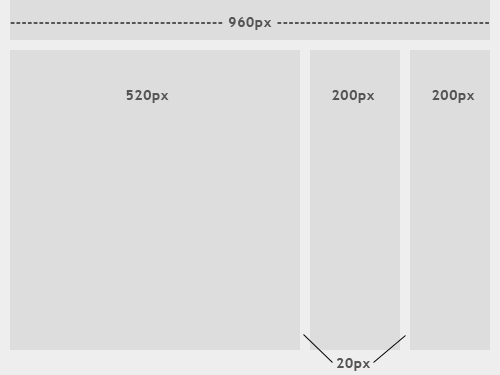
\includegraphics[scale=0.5]{images/image06.png}
	\end{center}
	\caption{Ukázka fixního layoutu\cite{fix}}
	\label{imgFix}
\end{figure}

%http://gs.statcounter.com/#resolution-ww-monthly-201204-201303

\textbf{Fluidní layout} neboli proměnlivý či tekutý layout (obr. \ref{imgFluid}) se typicky používá k~dosažení responzivního designu (vizte kapitola \ref{sec:rd}~Responzivní design). Jeho šířka se přizpůsobuje rozlišení zařízení. Elementy se nastavují v~procentech nebo \textit{em} jednotkách. Vnitřní a~vnější okraje (\textit{padding} a~\textit{margin}) se můžou nastavit fixně v~pixelech ale i~v~procentech. Častěji se využívá fixní šířka, neboť při velikém rozlišení při procentuálním vyjádření vznikají příliš velké mezery a~na malém zařízení jsou zase příliš úzké nebo obsah je těžce čitelný\cite{fix}.

\begin{figure}[h]
	\begin{center}
	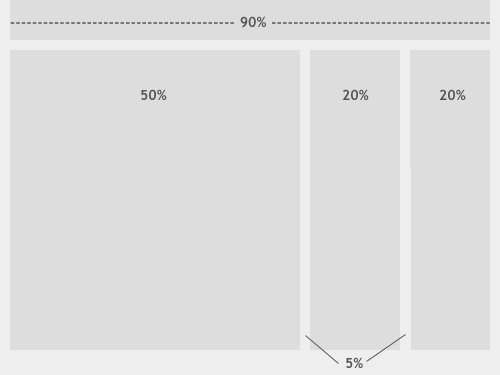
\includegraphics[scale=0.5]{images/image21.jpg}
	\end{center}
	\caption{Ukázka fluidního layoutu \cite{fix}}
	\label{imgFluid}
\end{figure}

Výhoda fluidního layoutu tkví ve flexibilnosti vůči nastavení uživatele včetně velikostí fontů. Kodér má ale menší kontrolu nad tím, co se uživateli zobrazí konkrétně a~v~některých rozlišeních může být vzniklý vzhled nežádoucí.

\textbf{Adaptabilní layout} řeší nedostatky fluidního layoutu, které se projevují při příliš nízkém či naopak vysokém rozlišení. Layout se adaptuje na tyto hraniční rozlišení díky využití \textit{media queries} (vizte následující kapitolu \ref{sec:rd}) nebo javascriptu. Při nízkém rozlišení navržený design vypadá příliš roztahaně a~naopak při extrémně velikém se kolem objevuje mnoho nevyužitého místa. Proto se ideálně navrhují např. tři základní rozložení - pro velmi malé displeje, pro klasické rozlišení obrazovek (např. u~notebooků) a~pro extrémně velké displeje\cite{adapt}.


\section{Responzivní web design} \label{sec:rd}


S pojmem \textbf{responzivní web design} přišel první Ethan Marcotte v~roce 2010 ve stejnojmenném článku na  A~List Apart. Vysvětluje, že při dnešní vysoké produkci všech možných zařízení (chytré telefony, tablety, čtečky knih), odkud lidé přistupují na webové stránky, je nezbytné, aby se web tomuto vývoji  přizpůsobil. V~dalších letech mobilní zařízení předstihnou desktopy a~najednou se nevyplatí vytvářet web zvlášť pro desktop a~navíc např. pro iPhone\cite{res}. Jeho předpověď se vyplnila velmi brzy. Dokazuje to statistický výzkum Googlu z~roku 2011. Na obrázku \ref{imgStatG} lze vidět, že lidé přistupují nejčastěji na internet ze svých přenosných zařízení. Jeví se to logicky, neboť uživatelé mají své zařízení stále u~sebe, takže mohou na internet přistoupit doslova kdykoliv.

\begin{figure}[h]
	\begin{center}
	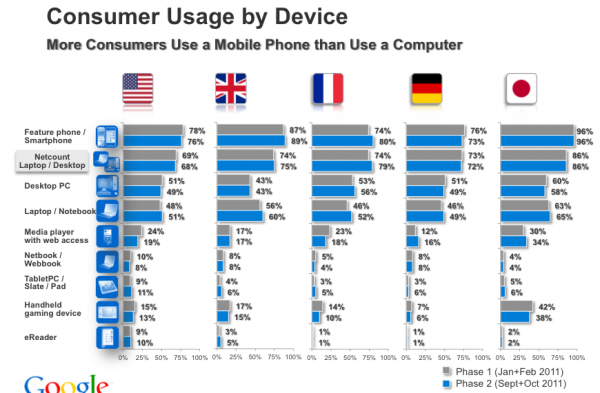
\includegraphics[scale=0.7]{images/image01.png}
	\end{center}
	\caption{Výsledky výzkumu o~přístupu na internet z~různých zařízení\cite{dev}}
	\label{imgStatG}
\end{figure}

A tady dostává své místo design přizpůsobující se rozlišení zobrazovacího zařízení neboli prohlížeči: \textit{responzivní web design}. Úzce souvisí právě s~tvorbou layoutů. Jedná se o~kombinaci fluidního a~adaptabilního layoutu. Základním pilířem responzivního designu je tzv. media query - specifikace CSS3, díky níž se definují rozdílné styly pro různá rozlišení. Použití v~praxi vypadá následovně:
\scriptsize
\begin{verbatim}
  @media all and (min-width:500px) { … }
  @media (min-width:500px) { … }
\end{verbatim}
\normalsize
Uvnitř bloku vymezeného složenými závorkami se definují vlastnosti, které se aplikují po splnění podmínky -- konkrétně minimální šířky prohlížeče na příslušném zařízení. Styly je možné různě propojovat a~strukturovat. Lze toho dosáhnout přímo v~\gls{HTML} dokumentu:
\scriptsize
\begin{verbatim}
  <link rel="stylesheet" type="text/css"
  media="screen and (max-device-width: 480px)"
  href="style480.css" />
\end{verbatim}
\normalsize
nebo v~\gls{CSS} souborech\cite{mq}
\scriptsize
\begin{verbatim}
@import url(style480.css) (min-width:480px);
\end{verbatim}
\normalsize


Responzivní design by měl také z~velké části být doménou samotných webových grafiků. Ti by měli být schopni navrhnout takový desgin, aby se při změně šířky vhodně adaptoval. Kodér naopak by měl znát jeho technické úskalí a~umět responzivitu reálně aplikovat. K~tomu znatelně pomáhají právě \gls{CSS} frameworky, zejména pak mřížkové (grid) systémy, které bez zohlednění responzivity jsou prakticky nepoužitelné\cite{dev}\cite{dev2}.

Otázka také je, zdali dnešní prohlížeče responzivní design vůbec podporují - tedy techniku CSS3 \textit{media queries}. Podle obrázku \ref{imgMQ} je to překvapivě vysoké procento a~v~podstatě jediné prohlížeče, které působí problém, jsou staré verze \gls{IE}\cite{mqsup}. 

\begin{figure}[h]
	\begin{center}
	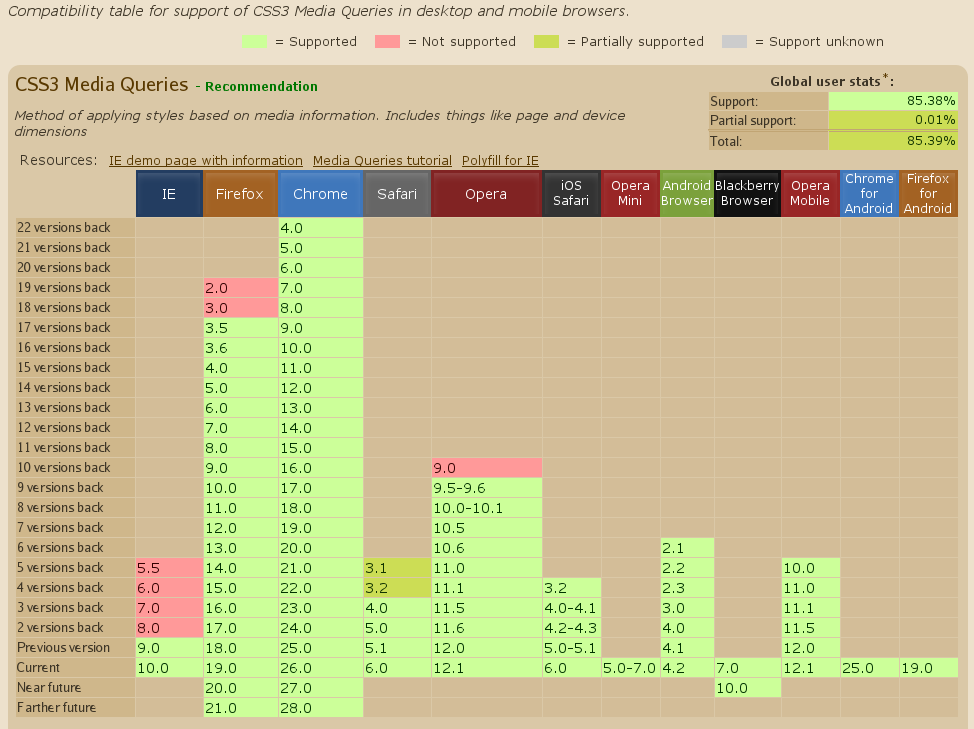
\includegraphics[scale=0.55]{images/image20.png}
	\end{center}
	\caption{Podpora media queries}
	\label{imgMQ}
\end{figure}


\newpage
\section{Typografie}


Typografie je neodmyslitelnou složkou celého webdesignu. Struktura textu má na výsledný dojem stejný podíl jako layout. Framework by měl vývojáři práci s~typografií usnadnit, ať už má nebo nemá vyloženě grafickou předlohu.

Typografická pravidla, kterých na webu lze dosáhnout, jsou zobrazení prvků jako uvozovky, pomlčky, rozdělovníky, mezery mezi navazujícími odstavci, vertikální mezery mezi nadpisy a~odstavci, odsazení prvního řádku. Některá nejsou možná zařídit kaskádovými styly jako např. odstranění jednoznakových předložek z~konců řádků. Ty se řeší až na úrovni samotného textu. Zbytek pravidel by však neměl být opomíjen.

Testování klade důraz na správné formátování odstavců a~nadpisů. Velikost fontu je možné relativně zvětšovat u~sémanticky významných prvků (nadpisů). Ovšem zmenšovat jej v~rámci běžných textů pod
preference uživatelů nedoporučuje. Plyne to z~doporučení \gls{W3C} o~přístupnosti webu.\cite{wcag} 

Jiný případ představuje řádkování. Řádky by od sebe měly mít nějaký odstup, který také není vhodný definovat fixně. Vůči nastavení uživatele to může být nedostačující nebo přehnané. Kdežto relativní jednotky zajistí formátování řádků vhodné přesně pro konkrétní nastavení. 

Mezi jednotlivými odstavci a~nadpisy by mělo být volné místo, aby záchytné body byly na první pohled patrné. Ostatní pravidla typografie ovlivní až vydavatel, který bude texty psát\footnote{V dnešní době se o~některá pravidla starají textové editory zabudované do redakčních systémů -- např. CKEditor.}. 



\section{Ovládací prvky a~formuláře}



Podpora ovládacích prvků je důležitá z~prostého důvodu -- málokterá webová stránka se bez nich obejde. Jedná se o~prvky, které uživatele nějakým způsobem navigují nebo mohou sami na stránce něco ovládat. Považovány jsou za ně tlačítka, různé druhy navigací, panel nástrojů, kontextová nápověda atd. Jejich stylování je přitom také časově náročná záležitost.  

Podpora všech těchto ovládacích prvků může být mnohdy nadstandardní ale pro někoho naopak nedostačující. Technicky je možné spojit více frameworků, pokud vývojář na stránce potřebuje širší škálu komponent. Tomuto účelu může posloužit např. knihovna Alloy UI , která je podrobněji popsána v~kapitole \ref{sec:boots}. Předpoklad testování je tedy zhodnocení základních ovládacích prvků, které jsou důležité a~potřebné téměř při každé stavbě webu:

\begin{itemize}
 \item navigace (i místní nabídka),
 \item tabulky,
 \item seznamy.
\end{itemize}

Samostatným kritériem jsou formuláře, jež se dají považovat za komponentu nadřazenou některým ovládacím prvkům. Jedná se o~textové oblasti (\textit{text area}), tlačítko pro odeslání (\textit{submit}), zaškrtávací pole (\textit{check box}), přepínače (\textit{radio button}), rozbalovací nabídka (\textit{select box}) a~případně další. Formuláře jsou nedílnou součástí objevující se na webu a~proto se předpokládá jejich podpora v~\gls{CSS} frameworcích.

\section{Soulad s~použitelností webu}
\label{sec:wcag}

V poslední řadě nelze opomenout použitelnost a~přístupnost webu, jak předkládá \gls{W3C} konzorcium. Z~velké části je to záležitost \gls{HTML} kódu, ale o~některé vlastnosti se zasluhují také kaskádové styly. \gls{CSS} frameworky by tuto použitelnost neměly porušovat. 

\gls{CSS} frameworky by měly obsahovat, pokud se jimi zabývají, následující vlastnosti:
\begin{itemize}
 	\item zřetelnou a~konzistentní navigaci (jednotná myšlenka designu),
 	\item elementy rozlišné barvy by měly svou informaci sdělovat i~bez barevného rozlišení,
 	\item možnost zobrazit obsah různými způsoby (např. jednodušší layout) bez ztráty informací nebo struktury.\cite{wcag}
\end{itemize}


\chapter{Testování frameworků}
Následující kapitoly rozšiřují jednoduché srovnání o~podrobnější poznatky než jsou shrnutí vlastností frameworků na internetu\footnote{Široké spektrum frameworků a~co podporují lze nalézt např. na webu \textit{Social~Compare} ze srpna 2012 \url{http://socialcompare.com/en/comparison/css-grids-amp-responsive-frameworks-comparison}.}. Také rozdělují frameworky  do skupin podle jejich zaměření. 
Kapitoly dále představí:

\begin{itemize}
  \item Použitelnost jednotlivých \gls{CSS} frameworků tak aby práce na webovém rozhraní byla:
	\begin{itemize}
 	\item jednoduchá a~pohodlná,
 	\item rychlá a~efektivní,
 	\item důsledná a~bez chybných zobrazení.
	\end{itemize}

 \item Jak si frameworky poradí s~jednotlivými kritérii a~jak jsou celkově použitelné pro:

\begin{itemize}
 \item e-shop (obsahují mnoho ikonek a~formulářů, mívají složitý layout),
 \item webový portál (vyžadují komplexní řešení, důležitá je typografie).
\end{itemize}
\end{itemize}
\section{Rozdělení frameworků podle zaměření}

\gls{CSS} frameworků se v~poslední době objevuje nepřeberné množství. Aby jim vývojáři lépe porozuměli, lze je rozdělit do typů podle jejich specializace:

\begin{itemize}
 \item mřížkové systémy,
 \item specializované typografické knihovny,
 \item komplexní frameworky.
\end{itemize}
Každou kategorii v~této práci zastupuje minimálně jeden \gls{CSS} framework. Pro komplexní frameworky je výzva shrnout všechny dobré praktiky používané na webu do jednoho celku. Ostatní zaměření frameworků mohou vývojářům velmi dobře posloužit ke konkrétním účelům. Jaké to jsou a~které frameworky jim odpovídají včetně zdůvodnění, proč byly zvoleny právě tyto, je uvedeno v~následující kapitole.


\section{Použitelnost CSS frameworků v~praxi}

\gls{CSS} frameworky, které jsou testovány v~této bakalářské práci, jsou následující:

\begin{itemize}
 \item Twitter Bootstrap,
 \item \gls{YAML} \gls{CSS} framework,
 \item 960~Grid System -- (specilizovaný na mřížkový systém),
 \item Baseline -- (specializovaný na typografii).
\end{itemize}
Komplexní framework Twitter Bootstrap představuje zajímavý objekt k~testování z~důvodu velké oblíbenosti mezi vývojáři. Kdo se alespoň okrajově setkal s~kódováním webových stránek, minimálně se o~něm doslechl. Přestože žádný framework nedosahuje takové popularity jako Bootstrap, je příhodné srovnat alespoň podobně vypracovaný framework a~zjistit, do jaké míry se mu svým charakterem může vyrovnat. Tento předpoklad splnil \gls{YAML} \gls{CSS} framework.

Frameworky, které jsou zaměřené na konkrétní oblast, se uplatní v~případě, kdy někteří vývojáři mají už své vlastní frameworky šité na míru např. specifickým potřebám ve své firmě. Komplexnost řešení dané problematiky ve frameworku by měla odpovídat vyšší úrovni než dosahují obecné frameworky. Předpokladem u~takových frameworků je také menší velikost zdrojových souborů a~s~tím související menší náročnost při načítání stránky.  

Předlohu pro testování frameworků \gls{YAML} a~Bootstrap představuje internetový obchod Alza.cz, který poskytuje dostatek potřebných prvků k~otestování a~jejich složitější rozestavění. Internetový obchod Alza.cz tak poskytl výborné prostředí pro zhodnocení, jak se určitý framework dokáže vypořádat s~takto komplexní aplikací.

Jako předloha pro typograficky zaměřený Baseline a~pro 960~Grid~System posloužil internetový hudební zpravodaj RollingStone.com. Na zpravodajských stránkách je dobrá typografie vyžadována více než na e-shopu (několik tisíc uživatelů čte denně články). Zpravodaj RollingStone.com  navíc obsahuje rozmanitý layout, který je skvělý k~otestování frameworku 960~Grid~System. 



\subsection{Postup práce}

S použitím konkrétního frameworku je cílem dosáhnout základního funkčního vzhledu zvoleného webu bez jediného zásahu do stylů. Znamená to, že bude vytvořeno jen \gls{HTML} s~třídami, jež framework nabízí. Z~toho vyplynou silné a~slabé stránky celého frameworku. 


\paragraph{Doporučení}

 \textit{Při kódování webových stránek je dobré využít styly, které upozorňují na některé nedostatky kódu. Lze použít již existující nástroj Diagnostic CSS\footnote{Ke stažení na \url{http://meyerweb.com/eric/tools/css/diagnostics/}.}. Díky nim vývojář na první pohled uvidí: }

\begin{itemize}
 \item \textit{nevyplněné atributy href, alt a~title,}
 \item \textit{\gls{HTML} značky bez obsahu (div, span, li, p, td, th),}
 \item \textit{nevyplněné atributy class a~id}.
\end{itemize}
\textit{Pokud není z~těchto vlastností nějaká v~pořádku, prvek se na stránce zvýrazní odlišnou barvou nebo se ohraničí. Ukazuje jednoduchý způsob, jak si ohlídat i~jiné vlastnosti na stránce. Tento nástroj se ukáže užitečný především v~době, kdy nám obsah generuje např. nějaký redakční systém a~uživatelé jej publikují pomocí editoru.}


\subsection{Způsob hodnocení frameworků}

Na závěr každého testování bude daný framework ohodnocen body podle zvolených kritérií. Hodnocení je shrnuto do tabulky následujícím způsobem:

\begin{itemize}
 \item 2 body: řešení je ideální a~bezchybné,
 \item 1 bod: kritérium je splněno, ale řešení není ideální nebo bezchybné,
 \item 0 bodů: framework neobsahuje požadované kritérium.
\end{itemize}
Čím větší získá framework ohodnocení, tím lépe splňuje kritéria a~je tedy z~hlediska testovaných kritérií kvalitnější.


\subsection{YAML CSS framework}

Přestože \gls{YAML} je zkratkou pro Yet Another Multicolumn Layout, tedy \quotedblbase ještě jiný vícesloupcový layout\textquotedblleft , dokáže konkurovat svou propracovaností i~frameworkům, které oficiálně nabízejí širší spektrum předpřipravených prvků. Tvůrce \gls{YAML}u \textit{Dirk Jesse} si správně uvědomil, že když už uživatel tvoří webové rozhraní, objeví se na něm i~formuláře, různé typy navigací a~tabulky. 

\gls{YAML} má dobře vyřešenou podporu prohlížeče \gls{IE}. Veškeré tyto tzv. \quotedblbase IE~hacky\textquotedblleft\footnote{Staré verze prohlížeče Internet Explorer jsou známé svým nedodržováním webových standardů. Odlišné zobrazení designu vývojáři řeší vkládáním identifikátorů před styly v~\gls{CSS} souborech, kterým rozumí pouze daná verze IE.} ukládá do samostatného souboru. Výhodu to představuje především pro vývojáře, kteří se rozhodnou cílit na skupinu používající moderní prohlížeče a~přejí si, aby zůstal web validní podle \gls{W3C} konzorcia. 

\paragraph{Responzivní web design}

\gls{YAML} si ve smyslu responzivity vede velmi dobře a~celková práce s~layoutem je více než pohodlná. Obsahuje jak fluidní, tak adaptabilní layout (obr.~\ref{imgYR}). Myšlenka adaptace layoutu je postavena na tzv. progresivní linearizaci. Znamená to, že není nutné vytvářet styly pro každé rozlišení zařízení zvlášť. Stačí určit hraniční šířku, od které layout vypadá nepoužitelně a~upravit třídy tvořící mřížku, aby se přizpůsobovaly aktuální šířce okna.


\paragraph{Layout}

Ve frameworku \gls{YAML} je možné volně kombinovat sloupcový systém s~mřížkovým systémem. Sloupcový systém poskytuje 1-3-2 nastavení. Sloupce 1 a~2 jsou definovány jako plovoucí prvky a~třetí představuje statický kontejner (obr.~\ref{imgCol}). Zastánci layoutu s~fixní šířkou 960~px (více v~kapitole \ref{sec:gs}) najdou ve frameworku také styly pro tento systém. 

V mřížkovém systému vývojář intuitivně použije správnou třídu pro šířku sloupce, kterou potřebuje, neboť její název vyznačuje určité procento. Pokud si vývojář přeje použít šířku jinou než \gls{YAML} nabízí, musí si takovou třídu vytvořit ve svém vlastním \gls{CSS} souboru.  

\begin{figure}[h]
	\begin{center}
	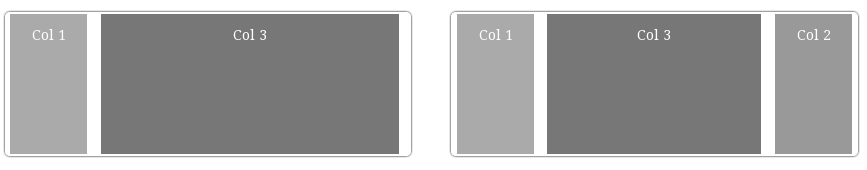
\includegraphics[scale=0.6]{images/image05.png}
	\end{center}
	\caption{Sloupce typu \quotedblbase 123\textquotedblleft \cite{yaml}}
	\label{imgCol}
\end{figure}

\paragraph{Typografie}

Jak si \gls{YAML} vyhrál s~grid a~column systémem, o~to méně si dal záležet na typografických zásadách. Všimnout si toho můžeme např. u~nadpisů. Na obrázku \ref{imgTyp} nadpis přes více řádků postrádá mezi řádky mezeru, aby byl nadpis lépe čitelný. V~tomto případě se řádky téměř slévají do sebe. Samozřejmě jde o~drobný nedostatek, který lze jednoduše zpravit ve svém vlastním \gls{CSS} kódu přidáním většího \verb#line-height#.

Když ale nahlédneme do zdrojových souborů, zjistíme, že výška řádků u~jednotlivých nadpisů je rozdílná a~ve většině případů nedostačující. U~nadpisu první úrovně je velikost písma 350~\% a~výška řádku je pouze 0.857~em. Celkově není jasné, podle jakých pravidel byly velikosti písem a~řádků stanoveny, každopádně čitelnosti neprospěly.

\paragraph{Ovládací prvky}

Dalším nedostatkem je malá flexibilita formulářových prvků. Celkově nelze dosáhnout klasicky používaných formulářových vzhledů, taktéž zaškrtávací pole (\textit{check boxy}) se správně neuspořádaly (obr.~\ref{imgCom}). 

\gls{YAML} poskytuje volby zarovnání, či nastavení obrázků, videí či dalších volitelných prvků i~jejich responzivní řešení. V~ohledu responzivity se jedná o~důležitý faktor, pro který by mělo existovat řešení, pokud je cílem práci vývojářům ulehčit. Za to patří \gls{YAML}u velké plus.


S ostatními ovládacími prvky nenastal žádný problém. U~tabulek  je možné vybírat ze tří stylů, což pro základní stavbu webu naprosto stačí. Dále nabízí navíc styly pro upozornění a~chybové hlášky plus další drobné prvky\footnote{Všechny si je lze prohlédnout v~online dokumentaci \url{http://www.yaml.de/docs/index.html}.}. 

\paragraph{Potenciál využití}

S ohledem na různé skupiny vývojářů bylo shledáno, že framework \gls{YAML} se skvěle hodí pro vývojáře, kteří webové stránky nikdy příliš nekódovali nebo chtějí rychle vytvořit funkční základ pro svou osobní prezentaci či jiný web a~nechtějí najímat drahé firmy. V~podrobné dokumentaci vývojář najde vše, co nabízí s~popisem, jak co použít včetně ukázkových \gls{HTML} kódů.

Zároveň framework může výborně posloužit i~větším webovým rozhraním, pokud se člověk chce zaměřit na detaily sám od začátku. Všechny základní principy použití jsou dostatečně vyřešeny a~dá se na nich stavět. 

Překážkou v~použití může být neexistující minimalizovaný soubor, který by měl obsah  všech \gls{CSS} souborů sjednotit. Dá se to vyřešit sice celkem snadno různými online minifikátory\footnote{Program, který zminimalizuje zdrojový kód např. do jednoho řádku. Jeden z~oblíbených se nachází na adrese \url{http://refresh-sf.com/yui/}}, ovšem hotový soubor ve frameworku by tento čas ušetřil. Další možností je použití preprocesoru \gls{Sass} nebo Stylus, které jedním příkazem zkompilují celý adresář a~zároveň soubory zminimalizují.

\paragraph{Hodnocení}

Kritéria hodnocení uvedená v~kapitole \ref{sec:hod} Kritéria a~hlediska testování byla pro názornost rozděleny do více podskupin. Dohromady získal \gls{YAML} 10~bodů z~12. Obsahoval všechny požadované styly. Ve dvou případech nebylo řešení úplně bezchybné.

\begin{table}[h]\centering
 	\caption[Hodnocení YAMLu]{Hodnocení frameworku YAML}\label{tab:yaml}
 	\begin{tabular}{|l|c|}\hline
 		\textbf{Kritérium} & \textbf{Body}\tabularnewline
  		\hline \hline
		Layout & 2\tabularnewline
		\hline 
		 Responsivní design & 2\tabularnewline
		\hline 
		Typografie & 1\tabularnewline
		\hline 
		Formuláře & 1\tabularnewline
		\hline 
		Ovládací prvky & 2\tabularnewline
		\hline 
		Media  (obrázky, videa,.. i~vzhledem k~RD) & 2\tabularnewline
		\hline 
		\textbf{Celkem} & \textbf{10}\tabularnewline
		\hline 
 	\end{tabular}
\end{table} 

\subsection{Twitter Bootstrap}
\label{sec:boots}

Bootstrap se oproti ostatním frameworkům stal robustním projektem, který si za dobu své krátké existence (necelé dva roky) získal širokou komunitu pomáhající s~vývojem. Cílovou skupinou tohoto frameworku se stali weboví vývojáři z~důvodu široké škály funkcí (existuje i~mnoho forků\footnote{Ve vývoji softwaru se forkem označuje případ, kdy vývojář vezme kompletní kód již existujícího programu a~začne na něm nezávisle vytvářet jiný program.} a~komponent), jež Bootstrap obsahuje. 

Propracovanost frameworku Bootstrap může být občas nevýhodou. Jelikož je v~něm vše vyřešeno, vývojáři se nechtějí dále zabývat grafickou stránkou projektu, a~tak weby ztrácejí svou jedinečnost.  Aby weby byly od sebe rozpoznatelné, dají se na ně aplikovat \textbf{témata} na tomto frameworku postavená.  Vývojář může vybírat ze zdarma open-source\footnote{Obrat open-source se používá v~souvislosti s~produkty, které mají veřejně dostupný zdrojový kód, podmínky užití se pak řídí danou licencí.} témat např. na stránce \url{http://bootswatch.com}. Mnohem lepší varianta se jeví zakoupit nějaké téma z~komerčních na stránce \url{http://wrapbootstrap.com/}, které tvoří profesionálové a~jejich výběr je pak daleko širší.

Bootstrap obsahuje ve výsledku dva nezminimalizované soubory s~\gls{CSS} styly. V~prvním souboru jsou uvedeny všechny styly v~jednom logickém celku, ve druhém se nacházejí styly pro vše, co souvisí s~reponzivím designem. Obsahuje tedy i~adaptabilní layout i~řešení responzivity obrázků, jak je viditělné na obrázku~\ref{imgB2} (pro obrázky existuje také několik dalších stylů).

Zdrojové soubory si lze stáhnout také rozdělené podle společných vlastností v~jednotlivých souborech, ale jsou napsány v~preprocesoru LESS. \gls{CSS} rozdělené soubory neobsahuje.


\paragraph{Layout}

Bootstrap užívá 12 sloupců, kde si vývojář volí mezi fixním a~fludiním layoutem. Poskytuje zanořování, takže nenastal případ, kdy by mezi jednotlivými elementy byly nežádoucí nebo chybějící mezery. 

\paragraph{Responzivní web design}

Layout se správně seskupil podle velikosti malého zařízení. Uživatel má nejdříve k~dispozici menu, aby se mohl přemístit, kam potřebuje (obr. \ref{imgB3}). Obrázky se automaticky zmenšují už na úrovni, jež nezahrnuje responzivní design.



\paragraph{Ovládací prvky}

Už na elementární úrovni člověk pozná, že se jedná o~komplexní framework. Obsahuje grafické rozhraní často pro nezbytné maličkosti jako je drobečková navigace nebo stránkovač (obr. \ref{imgB1}).

Všechny ostatní prvky, které bylo nutné použít k~postavení webového rozhraní Alzy, Bootstrap obsahoval v~daleko širším rozpětí, než bylo potřeba. (Bootstrap má podobně komplexní dokumentaci jako \gls{YAML}\footnote{Více informací o~všech podporovaných prvcích na oficiálním webu \\ \url{http://twitter.github.io/bootstrap/}.}) Pro oblasti formuláře, ovládací prvky i~media nabízel výběr hned mezi několika volbami -- např. navigace horizontální, vertikální, rozbalovací, přepínací záložky. V~kombinaci dvou voleb byla jednoduše vytvořena i~navigace v~e-shopu (obr.~\ref{imgNav}).

\paragraph{Potenciál využití}

 Bootstrap těžko využije webový grafik nebo obyčejný uživatel pro svůj blog. Nebude rozumět syntaxi preprocesoru LESS, v~němž je Bootstrap původně nakódován, a~v~konečném souboru obsahujícím všechny styly pohromadě se bude ztrácet. Na druhou stranu lze s~využitím různých komponent bez jediného zásahu do zdrojových souborů s~ním postavit celý web. 

\paragraph{Hodnocení}

Ve funkčním vzhledu není mezi Boostrapem a~ \gls{YAML}em příliš znatelný rozdíl. I \gls{YAML} je až na zmíněné nedostatky velmi dobře propracovaný. Jediný velký rozdíl mezi těmito frameworky je velikost komunity vyvíjející a~používající framework a~to především z~důvodu odlišné orientace každého frameworku.

Bootstrap se silně snaží o~dosažení dokonalosti a~není třeba zapírat, že se mu to dobře daří. Ve všech požadovaných kritériích dosahuje nejvyššího hodnocení. Znamená to, že pokud vývojář hledá framework, na který se může spolehnout ve všech důležitých i~méně používaných aspektech stránky, Bootstrap je pro něj tou nejlepší variantou.



\begin{table}[h]\centering
 	\caption[Hodnocení Bootstrapu]{Hodnocení frameworku Bootstrap}\label{tab:bootstrap}
 	\begin{tabular}{|l|c|}\hline
 	\textbf{Kritérium} & \textbf{Body}\tabularnewline
 	\hline\hline
		Layout & 2\tabularnewline
		\hline 
		 Responsivní design & 2\tabularnewline
		\hline 
		Typografie & 2\tabularnewline
		\hline 
		Formuláře & 2\tabularnewline
		\hline 
		Ovládací prvky & 2\tabularnewline
		\hline 
		Media  (obrázky, videa,.. i~vzhledem k~RD) & 2\tabularnewline
		\hline 
		\textbf{Celkem} & \textbf{12}\tabularnewline
		\hline 
 	\end{tabular}
\end{table} 

V souvislosti s~Bootstrapem stojí za zmínku ještě tzv. Alloy UI knihovna, jenž na něm staví a~obsahuje detailní komponenty jako např. hlasování pomocí hvězdiček, progressbar a~stromovou strukturu menu. Jedná se ovšem z~větší části o~javascriptovou knihovnu (obr.~\ref{imgAlloy}).

\begin{figure}[h]
	\begin{center}
	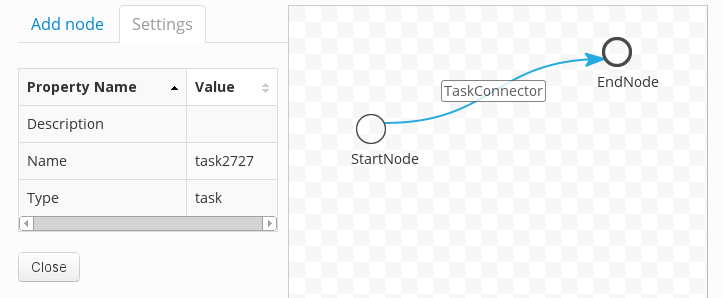
\includegraphics[scale=0.7]{images/image13.png}
	\end{center}
	\caption[Alloy UI komponenta]{Jednou z~nejnovějších komponent v~Alloy UI je např. Diagram Builder.}
	\label{imgAlloy}
\end{figure}

\newpage
\subsection{Baseline}

Baseline je framework postavený na myšlence účaří\footnote{Místo na které umisťujeme písmo např. v~sešitě je to linka.} v~typografii. Jde o~jakýsi “vertikální rytmus”, který uživateli v~jeho podvědomí napomáhá se na stránce orientovat. Baseline by měl zaručit, že ve všech sloupcích budou všechny velikosti fontů sedět na jednotné lince. Názorně je to předvedeno na obrázcích \ref{imgBa1} a~\ref{imgBa2}. 

\begin{figure}[h]
	\begin{center}
	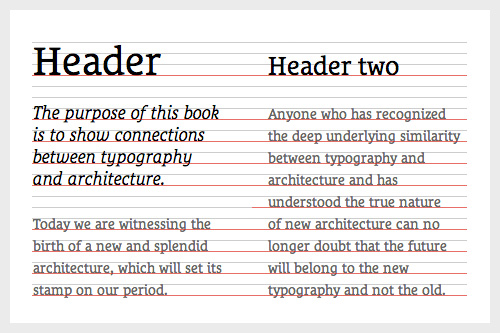
\includegraphics[scale=0.6]{images/image10.jpg}
	\end{center}
	\caption[Myšlenka účaří]{Všechen text zarovnán na jednu linku\cite{bas}}
	\label{imgBa1}
\end{figure}
\begin{figure}[h]
	\begin{center}
	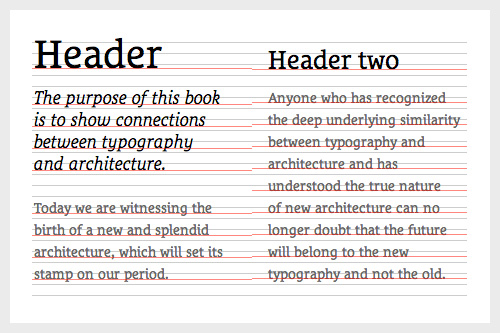
\includegraphics[scale=0.6]{images/image17.jpg}
	\end{center}
	\caption[Neuplatněná myšlenka účaří]{Text ve druhém sloupci odskakuje\cite{bas}}
	\label{imgBa2}
\end{figure}


Myšlenka účaří se ve webovém prostředí uplatňuje \cite{bas2}. Nutno však zmínit, že jde o~složitý vývoj vzhledem ke každému webu a~tudíž ji je vhodné použít spíše na menší weby, kde nebude příliš mnoho boxů. Pokud je typografie dobře nakódovaná, nic se nezmění ani při výměně fontu. Chtěl-li by ale někdo jiné proporce písma, musel by vytvořit nový koncept celého Baseline.

K hodnocení specializovaného frameworku jako je tento se musí přistupovat individuálním způsobem. Už na začátku jsme seznámeni s~tím, že v~rámci tohoto frameworku nejsou zhotoveny žádné navigační prvky, zvláštní ikonky a~tlačítka. Jeho hodnota by měla být někde jinde. Přesto obsahuje grid  systém, formuláře a~tabulky. Ze zvolených kritérií k~hodnocení bude ubrána položka responzivního designu.

\paragraph{Layout}

Baseline je omezující z~pohledu stavby layoutu. Při testování je nutné přizpůsobit frameworku výběr webu. Na webu RollingStone.com tedy nebyla brána v~úvahu úvodní strana, ale klasický dvousloupcový layout. Ten je typický právě pro zpravodajské weby a~blogy.

Při tvorbě webu si lze pomocí \gls{CSS} zobrazit mřížku \ref{imgBa3}, aby vývojář viděl a~kontroloval si, zdali je koncept účaří funkční a~něco jej nenarušuje. Kromě ní obsahuje framework ještě styly pro mobilní zařízení. Přestože nepočítá s~responzivním designem, je plusem, že myslí alespoň na mobilní zařízení. 



\paragraph{Typografie}

Problém nastane, když vložíme do stránek obrázek. Styly pro obrázky v~Baseline nejsou vůbec nijak předpřipraveny. Je to chybou, neboť rozhodí text tak, že přestane sedat na linky \ref{imgBa4}. V~tento okamžik přestává framework sloužit účelu, za jakým byl vytvořen. Přidání vlastnosti \verb#float: left# nebo \verb#right# vše napraví. Potenciálnímu vývojáři frameworku, který nemá s~kódováním příliš zkušenosti, to nemusí být ihned jasné. 

Baseline bohužel zmenšuje základní velikost písma, což odporuje zásadám použitelnosti podle \gls{W3C} standardu\cite{wcag}. Typografie pokulhává i~v~případě nadpisů a~odstavců. Pro odstavce používá knižní odsazení a~za odstavci nevkládá mezery. Odsazení je v~pořádku, ale nutno podotknout, že na webu se zvlášť při malé velikosti písma čte text bez mezery mezi odstavci hůře. Navíc u~nadpisů 5. a~6. úrovně nejsou mezery vůbec - ani nad ani pod nadpisem. Uživatel bude těžko tyto záchytné body považovat za nadpisy. Když zaměření padne jen na nadpis 6. úrovně, není rozeznatelný od textu označeného tučně tagem \verb#<strong></strong>#. Jsou to nedostatky, jež lze zpravit dodáním vlastního \gls{CSS}, jenomže tak může být lehce koncepce účaří rozbita.

\paragraph{Ovládací prvky}

Po zaměření na formulářové prvky nebyly shledány žádné nedostatky. Třídy používající se ke stavbě layoutu na různé šířky sloupců se univerzálně dají použít také na inputy, textarey, tabulky apod. Vývojář si tedy nemusí zapamatovávat hromadu názvů tříd.

\paragraph{Potenciál využití}

Framework má vysoký potenciál být rozšířenějším mezi vývojáři, kdyby věnoval svou pozornost více mřížkovému systému. Vytvoření více tříd, díky nimž nebude stavba tolik omezující jako nyní, by mu výrazně zvedlo preference.

Baseline najde své využití u~vývojářů, kteří nerozumí typografii nebo neumí její pravidla v~praxi aplikovat. Výrazně ulehčí práci také lidem, jež mají nějaké zkušenosti s~kódováním a~nepotřebují vytvářet složité webové rozhraní. Musí si ale dát pozor na to, aby nerozhodili koncept účaří, takže je dobré vědět, co jej ovlivní. Další skupinou lidí pro něž Baseline bude užitečný jsou vývojáři, kteří chtějí použít princip účaří jen s~jinými proporcemi písma. Najdou v~něm návod, jak správně tuto myšlenku realizovat.
\paragraph{Hodnocení}

Framework z~10 možných bodů (responzivní design nebrán v~úvahu) získal 6. Znamená to, že má v~lecčems hodně co dohánět. Autoři frameworku by si také měli ujasnit, na jakou skupinu vývojářů se chtějí zaměřit. Framework je postaven na opravdu dobré filozofii, která by měla být dotažena do nejmenších detailů. 

\begin{table}[h]\centering
 	\caption[Hodnocení Baseline]{Hodnocení frameworku Baseline}\label{tab:baseline}
 	\begin{tabular}{|l|c|}\hline
 	\textbf{Kritérium} & \textbf{Body}\tabularnewline
 	\hline\hline
		Layout & 1\tabularnewline
		\hline 
		 Responsivní design & -\tabularnewline
		\hline 
		Typografie & 1\tabularnewline
		\hline 
		Formuláře & 2\tabularnewline
		\hline 
		Ovládací prvky & 2\tabularnewline
		\hline 
		Media  (obrázky, videa,.. i~v0zhledem k~RD) & 0\tabularnewline
		\hline 
		\textbf{Celkem} & \textbf{6}\tabularnewline
		\hline 
 	\end{tabular}
\end{table} 

\subsection{960 Grid System} \label{sec:gs}

Jak už název~sám napovídá, jedná se o~framework obsahující styly pouze pro mřížkový (\textit{grid})  systém. Nezapomněl ale na typografické minimum a~nabízí také resetovací styly. Z~definovaných kritérií se testují pouze \textit{layout}, \textit{responzivní design} a~\textit{typografie}. Vývojáři tento framework rádi a~hojně používají díky vlastnosti čísla 960, proto byl výborný adept k~testování.

Koncept 960~px šířky vznikl primárně kvůli možnosti dělení čísla 960 mnoha čísly (2, 3, 4, 5, 6, 8, 10, 12, 15, 16, 20, 24, 30, 32, 40, 48, 60, 64, 80, 96, 120, 160, 192, 240, 320 a~480). Díky tomu je mřížka široká 960~px vysoce flexibilní vůči prvkům, které se na stránce vyskytují. Jak se k~tomu staví v~dnešní době tento systém, když rozlišení obrazovek stoupá, je popsáno níže.

\paragraph{Layout}

Framework ve své 960px šířce nabízí hned tři varianty -- 12, 16 a~24 sloupcový layout. Testovanému portálu RollingStone.com sedla lépe 12 sloupcová varianta. Kategorie Music vyžaduje dělení layoutu po 3 sloupcích (které jsou dále děleny opět na tři) nebo klasicky na jeden široký a~druhý uzší. V~16 sloupcové variantě je problém rozdělit již třetinu layoutu na další čitelné třetiny (vizte obr. \ref{imgGS1} a~\ref{imgGS2}).



960~Grid~System obsahuje ve stylech i~prefixy a~sufixy, jimiž si vývojář nadefinuje, zdali chce mít před nebo za sloupcem místo a~kolik přesně. Mezi jednotlivými řádky lze vložit tag \verb#<div># s~třídou \verb#.clear#, tak aby mezi boxy vznikla větší mezera.

\paragraph{Responzivní web design}

Jak bylo uvedeno v~kapitole o~responzivním designu, vývojáři čelí zařízením s~mnoha rozlišeními. V~této souvislosti je na místě položit si otázku, zdali legendární šířka 960~px bude pro web jako takový dostatečná. Závisí to na každém zvlášť, co je jeho preferencí. Chce-li však někdo používat pouze dobrý grid  systém, 960px šířka nemusí být překážkou. 

Framework nabízí řešení pro adaptivní layout\footnote{Na své hlavní stránce se odkazuje na \url{http://adapt.960.gs/}.}. Detekci šířky prohlížeče provádí pomocí javascriptu a~přiřazuje jim po té \gls{CSS} šité na míru. Šírky dělí na:

\begin{itemize}
 \item mobilní pod 760 px
(definuje pouze vnější okraje)
 \item 720 px u~rozlišení 760 px do 980 px
 \item 960 px u~rozlišení 980 px do 1280 px
 \item 1200 px u~rozlišení 1280 px do 1600 px
 \item 1560 px u~rozlišení 1600 px do 1940 px
 \item 1920 px u~rozlišení 1940 px do 2540 px
 \item 2520 px u~rozlišení nad 2540 px 
\end{itemize}

Kouzlo tkví v~návaznosti na samotný grid  systém. Stačí do hlavičky \gls{HTML} stránky přidat pár řádků a~okamžitě je stránka responzivní. Je to také příklad javascriptového řešení pro definování šířek k~docílení respozivního designu.
\scriptsize
\begin{verbatim}
<meta name="viewport" content="width=device-width, 
initial-scale=1, minimum-scale=1, maximum-scale=1" />


<script>
var ADAPT_CONFIG = {
  // Cesta k~CSS
  path: 'nathansmith-adapt-37a83aa/assets/css/',
  
  // false = Spustí se pouze jednou při načtení stránky
  // true = Mění se s~velikostí okna
  dynamic: true,
  
  range: [
     '0px to 760px  = mobile.min.css',
     '760px  to 980px  = 720.min.css',
     '980px  to 1280px = 960.min.css',
     '1280px to 1600px = 1200.min.css',
     '1600px to 1940px = 1560.min.css',
     '1940px to 2540px = 1920.min.css',
     '2540px           = 2520.min.css'
     ]
};
</script>
<script src="nathansmith-adapt-37a83aa/assets/js/adapt.min.js"></script>
\end{verbatim}
\normalsize


\paragraph{Typografie}
 Pokud se vývojář rozhodně používat čistě grid  systém, má k~tomu důvod, a~proto není potřeba vkládat do frameworku více, než je nezbytně nutné k~postavení slušného základu. 960 Grid System sice neobsahuje veliké množství stylů pro typografii, ale to by nebyl ten hlavní problém. Tyto styly pro typografii odporují zásadám použitelnosti webu podle kapitoly~\ref{sec:wcag}, neboť výška písma je definována fixně. Uživateli mohou zmenšit nastavení na jeho zařízení a zmenšit do takové velikost, až jej špatně uvidí.

\paragraph{Potenciál využití}

Framework 960 Grid System se hodí pro tři skupiny lidí. První jsou weboví vývojáři, kteří si potřebují jasně a~rychle navrhnout sloupcový systém a~pro ostatní prvky na webové stránky mají už vlastní framework. Nebo využívají či chtějí vyvíjet v~rámci své firmy framework pro své vlastní specifické potřeby a~potřebují kvalitní základnu v~podobě grid systému. Spíše ale než pro stavbu rozhraní by framework posloužil lépe webdesignerům. 

Druzí jsou grafici webových stránek, kteří spolupracují s~vývojáři a~dohromady se potřebují shodnout na jednotném smysluplném layoutu. 960~Grid System totiž poskytuje šablony pro grafické programy, které pomohou při návrhu layoutu. Patří mezi ně např. Adobe Photoshop a~InDesign, Gimp, Inkscape a~další. 

Třetí skupinou lidí mohou být začátečníci ve vývoji webového rozhraní. Díky frameworku se naučí používané návyky ve stavbě layoutu.


\section{Návrh a~realizace komponenty do~CSS~frameworků}


Vývoj webových technologií jde neustále kupředu a~pokud se přestanou vyvíjet, pro vývojáře přestanou být atraktivní a~užitečné. Nehledě na to, že potřebují mít jistotu, že technologie není zastaralá a~bude stále podporována. V~současných frameworcích, zejména pak ve frameworku Twitter Bootstrap, existuje mnoho komponent a~přibývají další. Při používání frameworků uživatel snadno narazí na něco, co mu schází a~co by mu usnadnilo práci.

\subsection{Návrh}

Při tvorbě stránek podle předlohy Alza.cz s~použitím frameworku \gls{YAML} a~Bootstrap vznikla potřeba nakódování reklamy kolem layoutu. Nic, co by usnadnilo reklamu vytvořit ani jeden z~frameworků nepodporuje. V~době, kdy vládne marketing a~firmy cítí nutnost propagovat své produkty na webových stránkách, je reklama často využívaným prvkem. Cílem bylo do těchto frameworků v~rámci bakalářské práce komponentu vytvořit a~zjistit, jak je to v~jeho rámci složité. Protože se nejedná o~specifický grafický prvek, nebyl problém s~designem daného frameworku.

Oba frameworky poskytují responzivní design a~pokud má být reklama cílená na všechny uživatele, je nutné, aby také odpovídala na aktuální šířku prohlížeče. Do frameworků byly navrženy celkem tři druhy reklamních bannerů (proužků). Vkládání bannerů se předpokládá do \gls{HTML} jako obrázek pomocí tagu \verb#<img />#, který může být obalený libovolnými značkami. Třídy se styly k~reklamě se nacházejí v~souboru \textit{adver.css}.

\subsection{Použití v~praxi}
Při tvorbě stylů byly v~úvahu brány konvence pojmenovávání daných frameworků. Každý element ve frameworku \gls{YAML} má prefix \quotedblbase ym-\textquotedblleft , v~Bootstrapu výrazná omezení v~pojmenování nejsou. 

Základem je horizontální banner, který může být umístěn kdekoliv na stránce (obr.~\ref{imgBan}). Pro zajištění správného chování v~případě řádkových (\textit{inline}) prvků, je potřeba tagu obsahující banner přidat třídu \verb#.ym-ad-hor# v~\gls{YAML}U a~v~Bootstrapu \verb#.ad-hor#. Jelikož \gls{YAML} poskytuje pro media třídu \verb#.flexible#, aby se banner přizpůsoboval šířce okna, stačí mu tuto třídu přiřadit. V~Bootstrapu toto není potřeba, neboť ten obrázky přizpůsobuje automaticky za každých podmínek.



Dalším využívaným prvkem k~upoutání pozornosti potenciálního zákazníka bývají bannery umístěné na bocích layoutu s~jejich fixní pozicí (obr.~\ref{imgFix}). Uživatel při skrolování stránky má banner stále na očích. Tagům obsahující tyto prvky se přiřadí třída \verb#.ym-ad-fix# nebo \verb#.ad-fix#. Přesné umístění banneru si uživatel musí definovat ale už sám podle rozmístění svého layoutu. 


Tento způsob umístění reklamy má význam pouze u~velkých rozlišení, kdy kolem layoutu existuje velká část prázdného místa. V~určitém okamžiku se okno prohlížeče nebo zařízení dostane do stavu, kdy samozřejmě boční bannery nebudou viditelné. Tehdy by se reklama měla umístit dovnitř layoutu (obr.~\ref{imgRes}), stejně jako to řeší samotná Alza.cz. Pro tento případ se použije horizontální varianta obrázku. V~\gls{HTML} dostane třídu \verb#.ym-ad-res# (\verb#.ad-res#), pro kterou je definován bod, v~němž layout nemá kolem sebe již dostatek místa na zobrazení bočních bannerů. Obrázek u~\gls{YAML}u by měl opět obsahovat třídu \verb#.flexible#.

\subsection{Zhodnocení}
Při porovnávání tvorby komponent pro každý framework zvlášť nebyly shledány výrazné rozdíly. Ve frameworku Bootstrap bylo jednodušší tvořit \gls{HTML} kostru, aniž by vývojář musel myslet na více tříd, které prvky potřebují mít přiřazené. Větší pozornosti a~znalost daného frameworku by byly potřeba, pokud by do něj vývojář chtěl více zasahovat. Platí podobná pravidla jako při vývoji softwaru. Svým zásahem lze nabourat navrženou koncepci.

Celkově vytvořit komponentu však nebylo nijak náročné. Lze předpokládat, že závislost na zdrojových souborech bude minimální i~při dalších možných komponentách.


\chapter{CSS preprocesory}
Přestože první preprocesory vznikly už před několika lety, jejich možnost využití se do většího podvědomí dostává kolem roku 2010. Internetové diskuse se plní debatami, zda použít \gls{CSS} preprocesor a~pokud ano, tak jaký. 

Důraz se klade na možnosti a~vhodnost nasazení z~hlediska syntaxe preprocesorového jazyka a~způsoby konverze do \gls{CSS}, případně další rozšiřující volby. Hodnotí se funkčnost a~varianty možného provázání do aplikací. Nakonec je popsána implementace napojení preprocesorů na redakční systém.


\section{Úvod do problematiky preprocesorů}


V momentu, kdy několik vývojářů pracuje na velikém projektu (pro představu např. Google nebo Facebook), okamžitě vývojář pozná sílu preprocesorů. Stejně jako v~programování se dnes používají zejména objektově orientované jazyky, přichází s~tímto i~komunita využívající \gls{CSS}. V~několika desítkách \gls{CSS} souborů už opravdu nastává obrovský chaos. \gls{CSS} preprocesory jsou pro něj jediným řešením.

Průkopníkem \gls{CSS} preprocesorů se stal jazyk \textbf{\gls{Sass}} vyvíjený od roku 2006. Z~něj si vzal inspiraci \textbf{LESS}, na němž se stále usilovně pracuje. S~novým a~vlastním neotřelým řešením přichází \textbf{Stylus}. Vytváří si vlastní konvence, s~nimiž může být obtížné se sžít, pokud jde o~konzervativní programátory. 

Existují i~další \gls{CSS} preprocesory, ale už nejsou tak dokonalé, nevyvíjejí se (např. xCSS\footnote{Tento preprocesor má kompilaci napsanou pouze v~\gls{PHP} \url{http://xcss.antpaw.org/}.}) anebo postrádají jakoukoliv~oficiální dokumentaci či rozumného průvodce. Kvůli uvedeným důvodům si u~vývojářů zatím nezískali tak vysokou popularitu.

Populární webový portál \textit{CSS Tricks} zabývající se \gls{CSS} vylepšeními v~roce 2012 uskutečnil anketu\footnote{Výsledky ke shlédnutí na \url{http://css-tricks.com/poll-results-popularity-of-css-preprocessors/}.}, kde zjišťoval, zdali návštěvníci využívají preprocesory a~pokud ano, tak jaké preferují. Odpovědělo téměř 13~000 návštěvníků. Mezi nejčastějšími odpovědmi se objevily právě tyto preprocesory. Přestože Stylus v~porovnání se \gls{Sass} a~LESS získal nízké procento úspěšnosti, nástroj vypadá dostatečně zajímavě na to, aby mu byla věnována pozornost. Před započetím prezentace poznatků je potřeba krátce uvést a~vysvětlit, jak se používají. 


\subsection{Sass}

Preprocesor \gls{Sass} je postaven na Ruby\footnote{Objektově orientovaný skriptovací programovací jazyk.}. Proto vývojáři, kteří jsou webové stránky zvyklí programovat v~Ruby on Rails\footnote{Framework nad jazykem Ruby používaný k~programování webových aplikací.}, nebudou mít problém s~nasazením, neboť se nemusí zabývat novými technikami. 

Jako běžná syntaxe se používá \quotedblbase SCSS\textquotedblleft   ~s rozšířením \verb#.scss# a~je nadmnožinou CSS3 syntaxe. Znamená to, že každé validní CSS3 styly jsou i~validní SCSS. Existuje i~starší syntaxe s~rozšířením \verb#.sass#. Hlavním rozdílem oproti SCSS je zjednodušený zápis -- není třeba používat závorky, středníky; místo toho se kód odsazuje a~zarovnává do bloků. Obě syntaxe jsou plně podporované.

\noindent Kód napsaný v~SCSS:
\scriptsize
\begin{verbatim}
 #main {
    color: blue;
    font-size: 0.3em;
 }
\end{verbatim}
\normalsize
Kód napsaný v~\gls{Sass}:
\scriptsize
\begin{verbatim}
 #main
    color: blue
    font-size: 0.3em
\end{verbatim}
\normalsize
K instalaci kompilátoru je nutné mít nainstalované Ruby, samotné stažení balíku a~instalace se provede příkazem:
\scriptsize
\begin{verbatim}
  gem install sass
\end{verbatim}
\normalsize
Překlad souborů se provede příkazem:
\scriptsize
\begin{verbatim}
  sass style.scss style.css
\end{verbatim}
\normalsize
(O kompilaci více v~kapitole \ref{sec:comp} Kompilace a~použití.)

\subsection{LESS}

LESS funguje jak s~kompilováním na straně serveru, tak s~javascriptem na straně klienta v~prohlížeči. Syntaxe je opět mezi LESS a~\gls{CSS} soubory přenositelná, ale na druhé straně vývojář nesmí žádné značení opomíjet. Může se to stát překážkou pro ty, kteří očekávají od preprocesoru ulehčení ve všech směrech včetně syntaxe. Na druhou stranu nedovolí vývojáři tvořit nečitelný kód.

\noindent Instalace se provede příkazem:
\scriptsize
\begin{verbatim}
  npm install -g less
\end{verbatim}
\normalsize
Kompilace pak:
\scriptsize
\begin{verbatim}
  lessc style.less style.css 
\end{verbatim}
\normalsize
případně nalinkováním souboru less.js dostupném na  oficiálním webu nebo Githubu\footnote{Jedná se o síť pro softwarový vývoj projektů jak open-source, tak komerčních.} projektu. Ukázka zavedení javascriptového překladu LESS souborů v~\gls{HTML}:
\scriptsize
\begin{verbatim}
<link rel="stylesheet/less" type="text/css" href="styles.less">
<script src="less-min.js" type="text/javascript"></script>
\end{verbatim}
\normalsize

\subsection{Stylus}

Stylus používá zjednodušenou syntaxi podobně jako \gls{Sass} s~rozdílem, že Stylus opomíjí všechny dělící znaky kromě čárek při výčtu hodnot:
\scriptsize
\begin{verbatim}
  body
    font 12px Helvetica, Arial, sans-serif

  a.button
    -webkit-border-radius 5px
    -moz-border-radius 5px
    border-radius 5px
\end{verbatim}
\normalsize
Nevýhodou této syntaxe je odsazování vlastností, podle kterého pozná i~zanořené elementy. Ovšem  je nutné dbát, aby v~celém dokumentu byly buď jen tabulátory nebo mezery. V~opačeném případě kompilace nebude fungovat. Pro vývojáře, kteří jsou tak zvyklí používat právě tabulátory k~odsazování, bude milejší pravděpodobně používání závorek. 

V preprocesorovém jazyce Stylus je klasická synaxe také možná. Lze používat jak závorky tak středníky a~dvojtečky. I když nebude dodržovaná, Stylus kompilaci zvládne. Ovšem otázkou je, jestli považovat za správné míchání syntaxe. Svádí potom ke kombinování a~opomíjení pravidel, což zhoršuje čitelnost kódu. Zjednodušený zápis kódu bez závorek se také hůře čte, navíc editory bez speciálních pluginů nezvládnou zvýrazňování syntaxe. Vyznat se v~takovém zápisu není jednoduché. Ale to také závisí především na osobních preferencích.

Stylus se intaluje se pomocí Node, podobně jako u~LESS:
\scriptsize
\begin{verbatim}
  npm install -g stylus
\end{verbatim}
\normalsize
Kompiluje se následujícím způsobem:
\scriptsize
\begin{verbatim}
  stylus style.styl style.css
\end{verbatim}
\normalsize


\section{Kompilace a~použití}
\label{sec:comp}


Všechny jazyky je třeba dostat do takové podoby, aby mu rozuměl sám prohlížeč. Ten neumí  preprocesorový jazyk interpretovat a~vykreslit, neboť mu nerozumí. Proto zdrojové soubory musí být zkompilovány a~toho se dá docílit třemi způsoby:


\begin{itemize}
 \item javascriptem,
 \item kompilací pomocí \gls{PHP},
 \item kompilátorem daného jazyka.
\end{itemize}

Používat kompilaci javascriptem v~produkčním režimu na webu není štastná volba. Při každé změně souboru se okamžitě na straně klienta změní i~obsah. Vhodné využití najde, když není žádoucí stále spouštět příkaz na kompilaci. V~případě LESSu nahradí chybějící volbu \verb#--watch#, jenž obsahují \gls{Sass} a~Stylus. Nicméně by bylo rozumnější tuto funkčnost minimálně zavést k~příkazu lessc oficiálně. Vývojář by si mohl vybrat, zdali chce používat javascript nebo bude využívat raději příkazovou řádku. 

\gls{PHP} kompilace je výhodná u~\gls{PHP} aplikací a~jejich frameworků, které nabízejí nějakou správu assetů\footnote{Statické soubory, které souvisejí s~tvorbou webové stránky jako např. obrázky, css soubory apod.}. Vývojáři pak nemusí používat nějaké další prostředí pro kompilaci preprocesorů a~vše se tak může dít automatiky. Díky \gls{PHP} parsování mohou být \gls{CSS} preprocesory integrovány do redakčních systémů či do \gls{PHP} frameworků, což je ukázáno v~kapitole \ref{sec:cms} Integrace preprocesorů do redakčního systému. 


Klasická kompilace na příkazové řádce se používá při vývoji na localhostu\footnote{Localhost odkazuje na místní počítač, kde běží program. Např. pokud je spuštěn webový prohlížeč na daném počítači, tento počítač je považován za localhost.}, kde má uživatel preprocesor nainstalovaný. Pokud vyvíjí webové rozhraní, použití této varianty je bezesporu nejvýhodnější. Samotný kompilátor obsahuje totiž několik užitečných nástrojů vývoj značně zpříjemňujících. 

\section{Hodnocení CSS preprocesorů}
Z důvodu markantnějších rozdílů mezi nástroji preprocesorů než mezi jejich samotnými funkcemi práce srovnává schopnosti jejich \textbf{nástrojů} vývoj ulehčit. U~každého nástroje je preprocesor zhodnocen 1 - 3 body vzhledem k~ostatním (3 je nejvíce) následujícím způsobem:

\begin{itemize}
 \item Pokud nástroj obsahuje každý z~preprocesorů, dostanou body podle jejich vhodnosti řešení (3,2 nebo 1). 
 \item Neobsahuje-li jeden preprocesor některý nástroj, ohodnocen bude 0 body, ostatní se mezi sebou rozdělí o~3 body. Pokud jsou nástroje rovnocenné, dostanou každý po 1 bodu.
 \item Poskytuje-li jen jeden preprocesor určitý nástroj a~ostatní ne, bude ohodnocen 3 body. 
\end{itemize}

\paragraph{Formát výstupu}

 U~preprocesoru \gls{Sass} si vývojář může zvolit formát výstupního souboru hned ze čtyř možných variant. Kromě komprese kódu do jednoho řádku lze vybrat formát s~viditelnou hiearchickou strukturou
\scriptsize
\begin{verbatim}
.ym-vlist {
  color: #00275a; }
  .ym-vlist ul {
    border-bottom: 0;
    border-top: 0; },
\end{verbatim}
\normalsize
s elementy rozdělěnými novým řádkem 
\scriptsize
\begin{verbatim}
.ym-vlist { color: #00275a; }
.ym-vlist ul { border-bottom: 0; border-top: 0; }
\end{verbatim}
\normalsize
nebo klasické rozmístění s~každou vlastností na samostatném řádku
\scriptsize
\begin{verbatim}
.ym-vlist {
  color: #00275a; }
.ym-vlist ul {
  border-bottom: 0;
  border-top: 0; }.
\end{verbatim}
\normalsize.

Naopak LESS nabízí kompresi YUI\footnote{Yahoo! User Interfece knihovna pro stavbu webových stránek. Mimo jiné poskytuje kompresor pro javascript a~css soubory \url{http://yui.github.io/yuicompressor/}.} či svou vlastní zjednodušenou kompresi. Stylus obsahuje volbu pouze zjednodušené komprese.\\
\gls{Sass}: 3, LESS: 2, Stylus: 1

\paragraph{Odlaďování chyb}

Pohodlné řešení debugovacího nástroje poskytuje LESS. V~konzoli při chybě překladu přímo zobrazí zvýrazněnou část kódu včetně čísla řádku, v~němž se nachází chyba i~s podáním vysvětlení. 

\begin{figure}[htb]
	\begin{center}
	\fbox{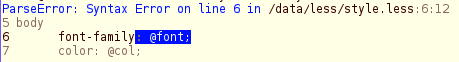
\includegraphics[scale=1]{images/image07.png}}
	\end{center}
	\caption{Ukázka upozornění preprocesoru LESS}
	\label{imgLESS1}
\end{figure}
Upozornění podobně řeší Stylus, občas ale nedokáže specifikovat jasně daný problém nebo také chybně, tak jako na obrázku. Za vlastností \verb#font-weight# chyběla hodnota, Stylus ale upozornil na špatné formátování.
\begin{figure}[h]
	\begin{center}
	\fbox{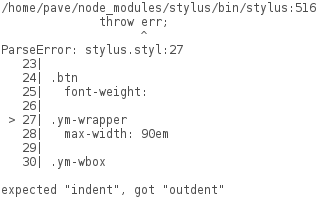
\includegraphics[scale=1]{images/image02.png}}
	\end{center}
	\caption{Ukázka upozornění preprocesoru Stylus}
	\label{imgSass1}
\end{figure}

Kdežto \gls{Sass} vypíše pouze vysvětlení chyby, která se nachází okolo určitého řádku, ale vždy to přesně nedokáže specifikovat. Znamená to, že se splete o~několik řádků. Všechny tři preprocesory pak obsahují debugovací nástroje pro prohlížeč Firefox -- \textit{FireSass}, \textit{FireLESS} a~\textit{FireStylus}.\\
LESS: 3, Stylus: 2, \gls{Sass}: 1

\begin{figure}[h]
	\begin{center}
	\fbox{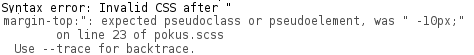
\includegraphics[scale=1]{images/image22.png}}
	\end{center}
	\caption{Ukázka upozornění preprocesoru Sass}
	\label{imgStyl1}
\end{figure}


\paragraph{Hromadná kompilace a~sledování změn}

 \gls{Sass} a~Stylus obecně nabízí širší škálu nástrojů. Navíc obsahují např. hromadnou kompilaci css souborů v~určitém adresáři nebo sledování změny souboru, kdy se příkaz na kompilaci spustí jen jednou:
\scriptsize
\begin{verbatim}
sass --watch style.scss:style.css
stylus --watch style.styl:style.css
\end{verbatim}
\normalsize
\gls{Sass}: 1, Stylus: 1, LESS: 0

\paragraph{Zaokrouhlování}

 Při matematických operacích \gls{Sass} poskytuje volbu přesnosti zaokrouhlení u~desetinných míst. Toto se užitečné jeví především při použití fluidního layoutu.\\ 
\gls{Sass}: 3, LESS: 0, Stylus:0
\paragraph{Konverze do vlastní syntaxe}

 Všechny tři preprocesory umožňují dokonce konverzi \gls{CSS} do své syntaxe, ale žádný nenahradí opakované hodnoty např. proměnnými. Stylus nezanořuje bloky do sebe.
\scriptsize
\begin{verbatim}
stylus --css < test.css > test.styl
\end{verbatim}
\normalsize
LESS tento nátroj zvaný LESSify\footnote{Na internetu je dostupný online konvertor \url{http://leafo.net/lessphp/lessify/}.} oficálně nepodporuje. Jde zatím o~vývojovou verzi, ale oproti preprocesoru Stylus dokáže rozpoznat bloky, které k~sobě patří a~zanořit je. To už je mnohem použitelnější, potřebuje-li vývojář přenášet různé styly např. z~dřívějších projektů. 
\gls{Sass} umí také zanořovat, pokud \gls{CSS} soubor obsahuje komentáře, kompilátor se s~ním bezchybně nepopere. Sice vše zanoří správně, ovšem způsobí zakomentování celého kódu od bloku, kde se poprvé vyskytl. Bohužel také konvertuje do syntaxe bez závorek a~středníků, což může být pro někoho překážka. 

\scriptsize
\begin{verbatim}
sass-convert test.css test.scss
\end{verbatim}
\normalsize
LESS:3, \gls{Sass}: 2, Stylus:1
\paragraph{Interaktivní režim}

 Za zmínku stojí interaktivní mód, jenž nabízí Stylus. Na příkazové řádce lze na výstupu dostat, jak bude např. vypadat určitá barva:
\begin{figure}[h]
	\begin{center}
	\fbox{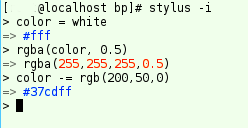
\includegraphics[scale=1]{images/image18.png}}
	\end{center}
	\caption{Interaktivní mód preprocesoru Stylus}
	\label{imgStyl2}
\end{figure}

\noindent Stylus: 3, \gls{Sass}: 0, LESS: 0



\begin{table}\centering
 	\caption[Hodnocení preprocesorů]{Hodnocení preprocesorů}\label{tab:pre}
 	\begin{tabular}{|l|c|c|c|}\hline
	\textbf{Kritérium} & \textbf{Sass} & \textbf{LESS} & \textbf{Stylus} \tabularnewline	
 	\hline\hline
		 Formát výstupu & 3 & 2 & 1\tabularnewline\hline
		 Odlaďování chyb & 1 & 3 & 2\tabularnewline\hline
		 Hromadná kompilace a~sledování změn & 1 & 0 & 1\tabularnewline\hline
		 Zaokrouhlení & 3 & 0 & 0\tabularnewline\hline
		 Konverze do vlastní syntaxe & 2 & 3 & 1\tabularnewline\hline
		 Interaktivní režim  & 0 & 0 & 3\tabularnewline\hline
		 \textbf{Celkem} & \textbf{10} & \textbf{8} & \textbf{8}\tabularnewline\hline
 	\end{tabular}
\end{table} 


\paragraph{Hodnocení}

Z výsledného hodnocení plynou dvě věci. Za prvé, jde vidět, že \gls{Sass} se vývoji věnuje již několik let a~obsahuje oproti ostatním nejvíce nástrojů z~hodnocených. Za druhé, LESS dokazuje, že i~když má nástrojů oproti konkurentům méně, jsou použitelnější a~uživatelsky přívětivější. Stylus má ve kvalitě co dohánět, ale je na slibné cestě (tab. \ref{tab:pre}).




\section{Integrace CSS preprocesorů do CMS systému}
\label{sec:cms}

Na poli redakčních systémů neboli \gls{CMS} existují implementace kompilátoru \gls{CSS} preprocesorů uvnitř systémů, ale lze je najít i~v~samotných \gls{PHP} frameworcích (např. Symfony). Pro účely této bakalářské práce byl vybrán open source redakční systém Venne:CMS\footnote{Celý projekt i~s moduly je volně ke stažení na \url{http://github.com/venne}.} (dále jen Venne). Tento redakční systém postavený na Nette frameworku se vyznačuje vysokou modularitou a~cílením jak na uživatele, tak samotné vývojáře.



\subsection{Motivace}

Integrovaný \gls{CSS} preprocesor umožní psát styly v~dynamickém jazyce pro šablony přímo v~\gls{CMS} tak, aby kompilace mohla probíhat přímo online na daném hostingu. Je možné tedy měnit styly pro webové rozhraní přímo ve vybraném preprocesorovém jazyce. 

Jako užitečná pomůcka se to projeví zejména ve chvíli, kdy správce webu nemá u~sebe svou vývojovou verzi a~je nutné rychle zasáhnout a~opravit nějakou chybu či nedostatek. V~opačném případě na localhostu usnadní vývojáři čas tím, že nemusí stále spouštět příkaz na kompilaci souborů při každé malé změně. Modul to vyřeší za něj. 



\subsection{Realizace}

K vytvoření jednotlivých modulů, které nám zajistí kompilaci potřebujeme \gls{PHP} kompilátor pro daný preprocesor. Tyto kompilátory dnes pro \gls{Sass} i~LESS existují. U~LESS je to \textit{lessphp} a~u \gls{Sass} \textit{phpsass}. Pro Stylus zatím php kompilátor neexistuje.
 
Základem modulu ovládající kompilaci je vytvoření makra fungujícího v~šablonovacím systému \gls{CMS}. Syntaxe makra byla zvolena obdobná, jako u~maker \textit{css} a~\textit{js}, které jsou standardně dostupné:
\scriptsize
\begin{verbatim}
{pojmenovani_makra @NazevModul/cesta_k_souboru/nazev_souboru.pripona}
\end{verbatim}
\normalsize

Označením \verb#@NazevModul# v~tomto případě rozumíme modul pro konkrétní webovou stránku, ve kterém se nachází zejména  šablona a~dále všechny potřebné soubory k~zobrazení layoutu a~rozhraní stránky - tzn. obrázky, styly, fonty a~nyní i~soubory preprocesorového jazyka. Cesta k~souboru se určuje absolutně od tohoto modulu až k~samotnému souboru\cite{ven}. 

Aby byly dodrženy určité dobré zvyky a~důslednost v~daném redakčním systému, do implementace bylo zahrnuto vytváření adresáře v~mezipaměti, kam se následně zkompilovaný soubor ukládá. Není totiž žádoucí, aby se soubor kompiloval při každém načítání stránky, ale pouze při kompilaci šablony, kde je umístěné zmíněné makro. (Uvažujeme-li však nastavení \gls{CMS} v~debugovacím módu, makro rozliší tuto skutečnost a~zkompiluje less soubory vždy při změně \gls{CSS} souboru.)  

Část názvu souboru se vygeneruje jako hash cesty k~souboru a~data poslední změny. Toto nám zaručí unikátní název~souboru. Nestane se, aby se do adresáře umístily dva shodně nazvané soubory a~jelikož celá cesta k~souboru může být příliš dlouhá, vyřeší toto hash. Hash se vygeneruje vždy stejně dlouhá.

V debugovacím módu při změně souboru je starý nepotřebný soubor se styly odstraněn díky druhé hashi v~názvu. Aby vývojář sám byl schopen poznat o~který soubor se jedná, na začátku názvu je umístěn původní název souboru - např. \textit{style.less}.



\subsection{Modul LESS}\footnote{Volně dostupný ke stažení na \url{http://github.com/venne/less-module}.}

V případě makra pro less soubory bude zápis v~šabloně vypadat následovně:
\scriptsize
\begin{verbatim}
{less @NazevModul/cesta_k_souboru/style.less}
\end{verbatim}
\normalsize
Po kompilaci less souboru a~zpracování makra dostaneme v~\gls{HTML} stránce nalinkovaný css soubor:
\scriptsize
\begin{verbatim}
<link rel="stylesheet"
href="/www/cache/less/styl.less-hash1-hash2.css" type="text/css" />
\end{verbatim}
\normalsize
Implementace LESS makra pak závisí na dvou nejdůležitějších krocích:

\begin{itemize}
 \item vytvoření instance less kompilátoru
 \item příkazu zařizujícím samotnou kompilaci na základě vstupního souboru
\end{itemize}
\scriptsize
\begin{verbatim}
//vytvoření instance kompilátoru
$less = new \lessc(); 
//metoda kompilující soubor $in do souboru $out, 
//kde $in a~$out jsou absolutními cestami souborů
$less->compileFile($in, $out); 
\end{verbatim}
\normalsize
Jelikož se redakční systém Venne dá ovládat z~příkazové řádky (má v~sobě zabudovanou konzoli z~frameworku Symfony), do modulu byl implementován také příkaz, který kompilaci zajistí bez nutnosti instalace kompilátoru LESS do uživatelova počítače\footnote{Vytvořeno podle manuálu \url{https://github.com/Venne/venne-docs/blob/master/framework/commands.md}}. Implementace je poněkud jednodušší, kompilaci je však nutné ošetřit vyhozením výjimky a~informováním uživatele o~případné chybě:
\scriptsize
\begin{verbatim}
$less = new \lessc();
try {
   $less->compileFile($in, $out);
} catch (\Exception $e) {
   // příkaz, který na konzoli vypíše, kde se v~souboru stala chyba
   $output->writeln("<error>fatal error: {$e->getMessage()}</error>"); 
}
\end{verbatim}
\normalsize
V případě makra se toto řešit nemusí, neboť Nette vyhazuje výjimky automaticky v~nástroji zvaném Tracy (dříve Laděnka).



\subsection{Modul Sass}

Logika zpracování souboru s~obsahem preprocesorového jazyka bude při zavedení podpory každého dalšího procesoru stejná. Lišit se bude v~kompilovacím příkazu a~drobnostech, které implementace jednotlivého parseru odlišuje. U~\gls{Sass} makra použijeme následující:	

\scriptsize
\begin{verbatim}
//metoda toCss vrací string výsledného css obsahu
$css = $sass->toCss($path); 
//css obsah vložíme do souboru nacházející se na absolutní adrese uložené 
//v proměnné $out
file_put_contents($target, $css);  
\end{verbatim}
\normalsize
Implementace příkazu kompilující scss nebo sass soubory bude postavena na kombinaci logiky v~LESS modulu a~výše uvedených řádků:
\scriptsize
\begin{verbatim}
$sass = new \SassParser(); //vytvoření instance kompilátoru
try {
   $css = $sass->toCss($in); 	
   file_put_contents($out, $css);
} catch (\Exception $e) {
   $output->writeln("<error>fatal error: {$e->getMessage()}</error>");
}
\end{verbatim}
\normalsize
Uživatelé redakčního systému, kteří si přejí používat k~vývoji \gls{CSS} preprocesor mají nyní na výběr z~LESS nebo \gls{Sass} jazyka podle jejich vlastních preferencí. Oba z~modulů jsou dostupné na Githubu\footnote{LessModule: \url{http://github.com/venne/less-module}, \\SassModule: \url{http://github.com/venne/sass-module}}. Do budoucna se určitě počítá s~vytvořením i~modulu pro Stylus, jakmile se pro něj objeví \gls{PHP} kompilátor.


\begin{conclusion}
	Čtyři různé CSS frameworky mi rozšířily obzory a~poskytly znalosti, na kterých bude snadné stavět další. Zjistila jsem, že na počátku každého projektu automaticky vzniká potřeba ujasnit si kritéria, která webové rozhraní má slpňovat a~která očekávám od použitých nástrojů. 

Technologie se navzájem doplňují a~podporují jedna druhou. Proto i~v~této práci byla snaha zaznamenat souvislosti mezi CSS preprocesory a~frameworky. Čím více jsou technologie mezi sebou podporované, tím více vývojáři usnadní práci. Vývojáři často argumentují výtkami, jimiž obhajují, proč nepoužívají modernější nástroje. Tato práce však většinu dokázala vyvrátit pouhými zjištěnými poznatky, což považuji za úspěch. 

Bakalářská práce je pouhým odrazem v~dané problematice. Preprocesory a~frameworky mi přišla natolik zajímavá, že v~jejím zkoumání neustanu, budu otestované sledovat a~další zkoušet a~používat.  

\end{conclusion}

\bibliographystyle{csn690}
\bibliography{mybibliographyfile}

\appendix
\chapter{Obrázky}

\begin{figure}[h]
	\begin{center}
	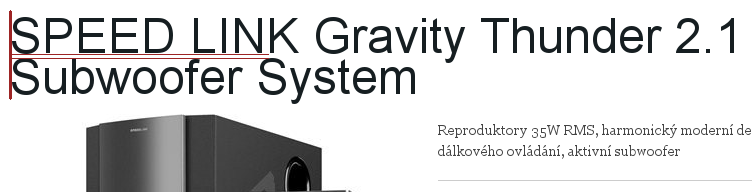
\includegraphics[scale=0.7]{images/image04.png}
	\end{center}
	\caption[Nedokonalá typografie u~frameworku YAML]{Nedokonalá typografie u~frameworku YAML: Mezera mezi řádky nadpisu je téměř neznatelná.}
	\label{imgTyp}
\end{figure}

\begin{figure}[h]
	\begin{center}
	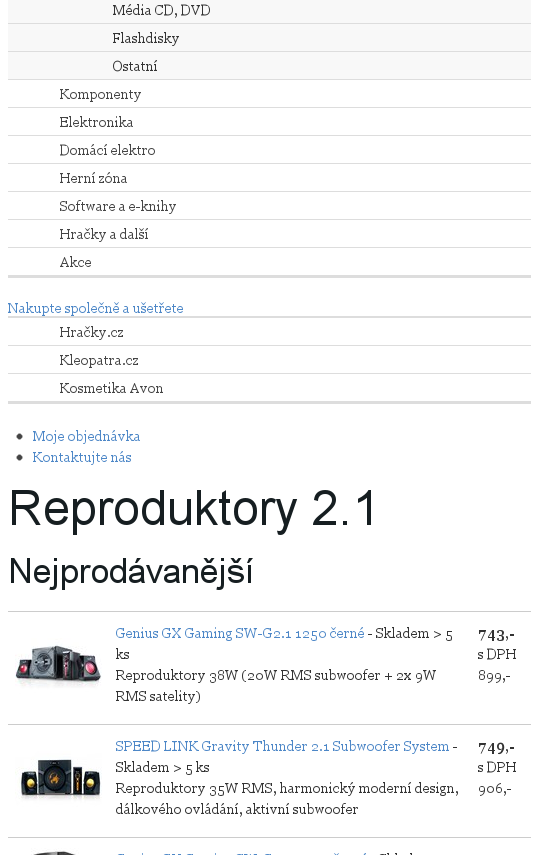
\includegraphics[scale=0.7]{images/image16.png}
	\end{center}
	\caption{Responzivní web pomocí frameworku YAML}
	\label{imgYR}
\end{figure}


\begin{figure}[h]
	\begin{center}
	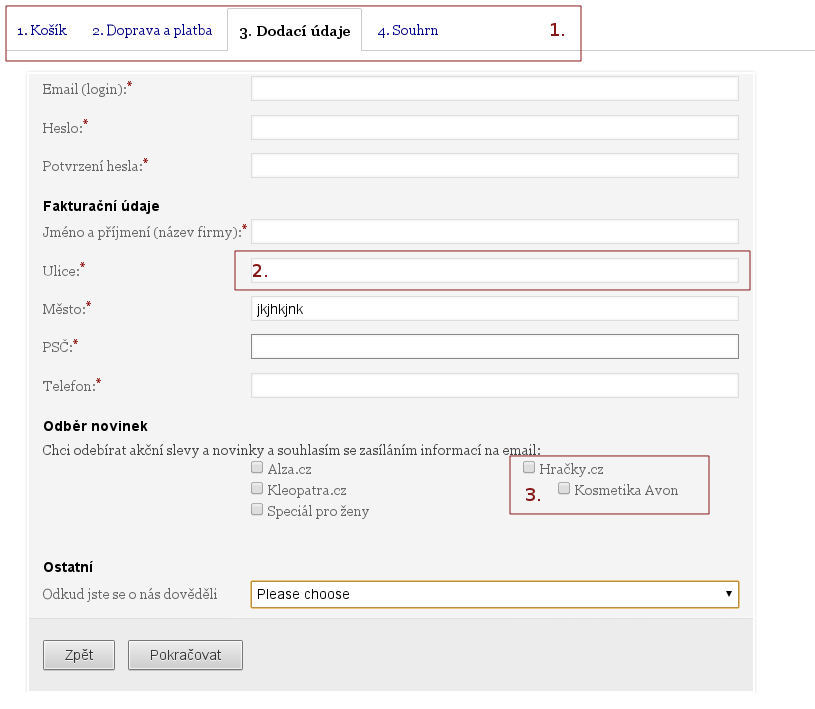
\includegraphics[scale=0.7]{images/image19.png}
	\end{center}
	\caption[Poznatky týkající se frameworku YAML]{Poznatky týkajjící se frameworku YAML: 1.~Přestože je YAML primárně grid  systém, obsahuje i~pohodlné javascriptové přepínání záložek. 2.~Bohužel YAML nabízí pouze tři základní délky inputů ve formuláři. Není tedy příliš přizpůsobivý potřebám uživatele. 3.~Přestože do \gls{CSS} nebylo nijak zasahováno a~\gls{HTML} standardně použito podle předpokladů YAML, checkboxy se rozmístily do nového sloupce křivě.}
	\label{imgCom}
\end{figure}

\begin{figure}[h]
	\begin{center}
	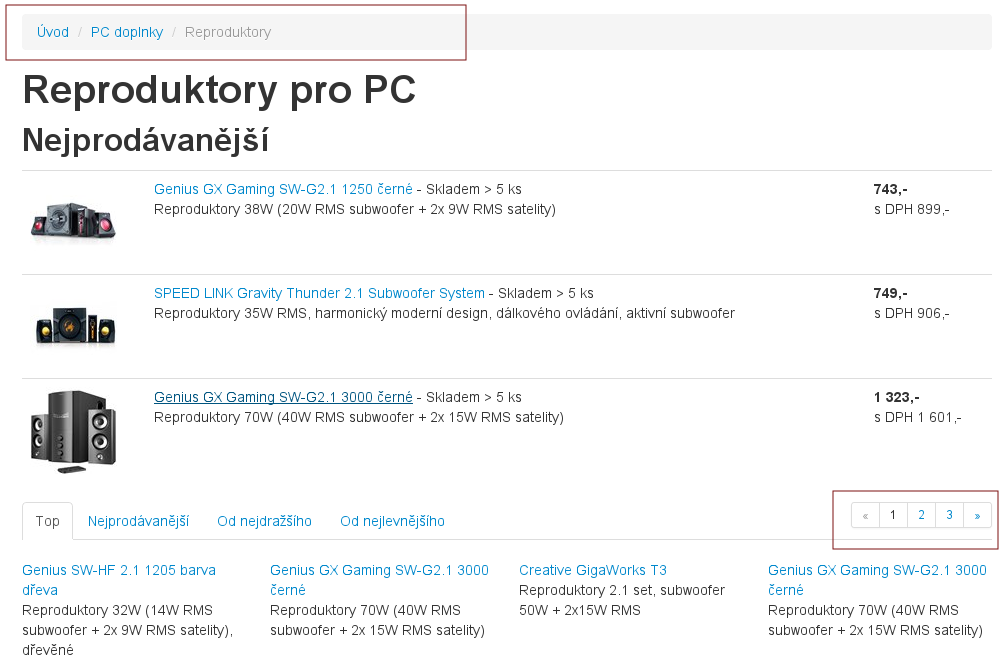
\includegraphics[scale=0.5]{images/image08.png}
	\end{center}
	\caption{Ukázka použitých komponent Bootstrapu}
	\label{imgB1}
\end{figure}

\begin{figure}[h]
	\begin{center}
	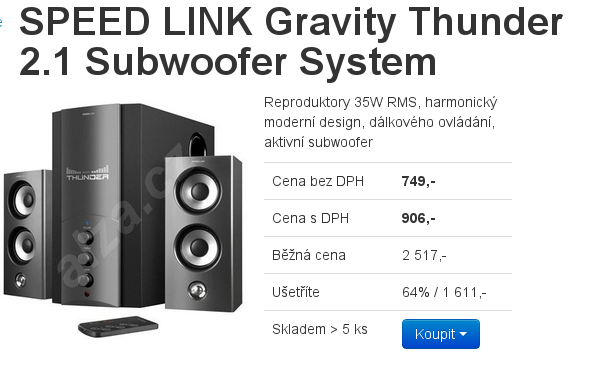
\includegraphics[scale=1]{images/image15.png}
	\end{center}
	\caption[Flexibilní obrázek ve frameworku Bootstrap]{Flexibilní obrázek ve frameworku Bootstrap: screen obrazovky v~originální velikosti s~přizpůsobeným obrázkem.}
	\label{imgB2}
\end{figure}

\begin{figure}[p]
	\begin{center}
	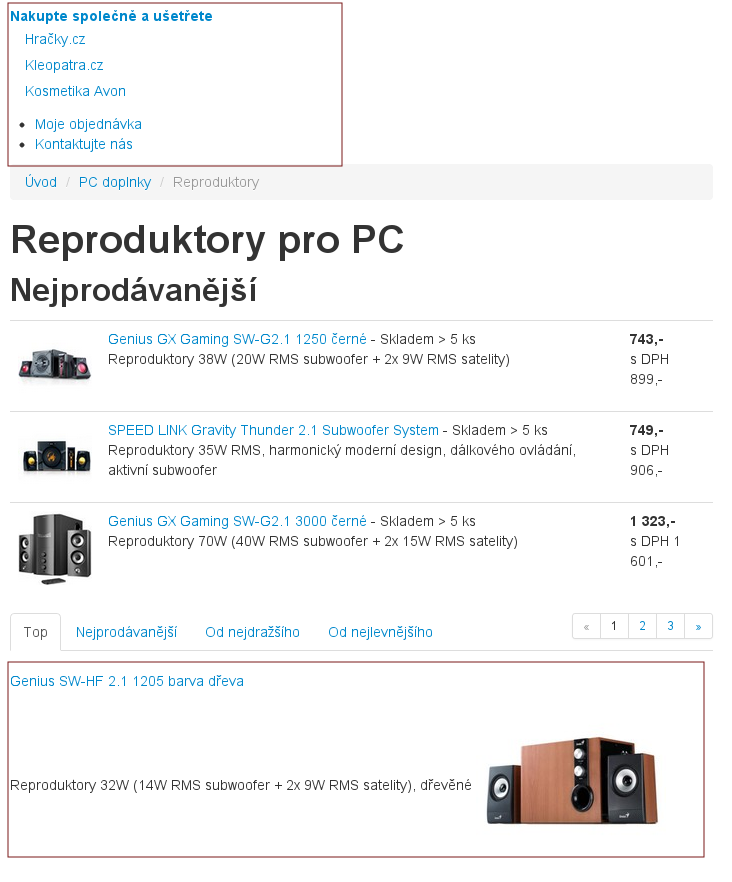
\includegraphics[scale=0.7]{images/image11.png}
	\end{center}
	\caption{Responzivita frameworku Bootstrap}
	\label{imgB3}
\end{figure}

\begin{figure}[htb]
	\begin{center}
	
\includegraphics[scale=1]{images/image00.png}
	\end{center}
	\caption{Bootstrap: Navigace v~nákupním košíku podle předlohy Alza.cz}
	\label{imgNav}
\end{figure}

\begin{figure}[h]
	\begin{center}
	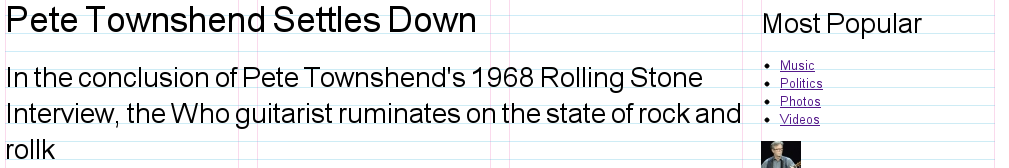
\includegraphics[scale=0.5]{images/image14.png}
	\end{center}
	\caption{Ukázka zobrazení mřížky na stránce v~Baseline}
	\label{imgBa3}
\end{figure}

\begin{figure}[h]
	\begin{center}
	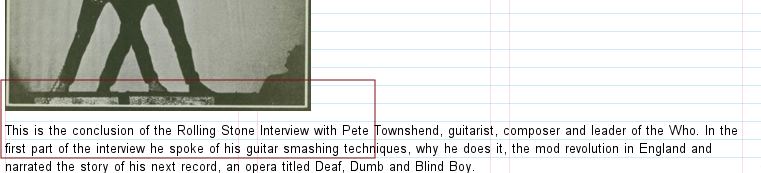
\includegraphics[scale=0.7]{images/image03.png}
	\end{center}
	\caption{Baseline: Rozhozená koncepce účaří}
	\label{imgBa4}
\end{figure}

\begin{figure}[h]
	\begin{center}
	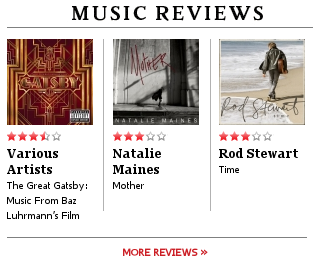
\includegraphics[scale=1]{images/image12.png}
	\end{center}
	\caption{Předloha z~RollingStone.com pro vytvoření 3 sloupců v~jednom}
	\label{imgGS1}
\end{figure}
\begin{figure}[h]
	\begin{center}
	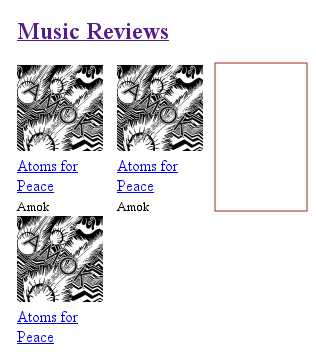
\includegraphics[scale=1]{images/image09.png}
	\end{center}
	\caption[Využití 960 Grid System]{960 Grid System: Ve sloupci už nezbylo místo na poslední položku podle předlohy}
	\label{imgGS2}
\end{figure}
\begin{figure}[h]
	\begin{center}
	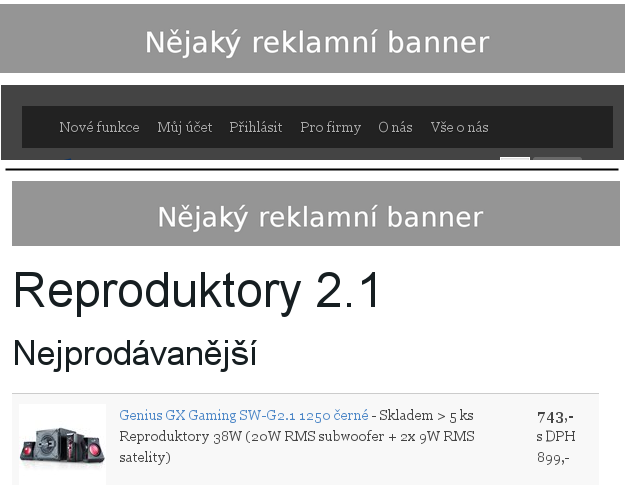
\includegraphics[scale=0.6]{images/image23.png}
	\end{center}
	\caption[Horizontální banner]{Komponenta: Libovolný horizontální banner kdekoliv na stráce s~libovolnou šířkou okna.}
	\label{imgBan}
\end{figure}
\begin{figure}[h]
	\begin{center}
	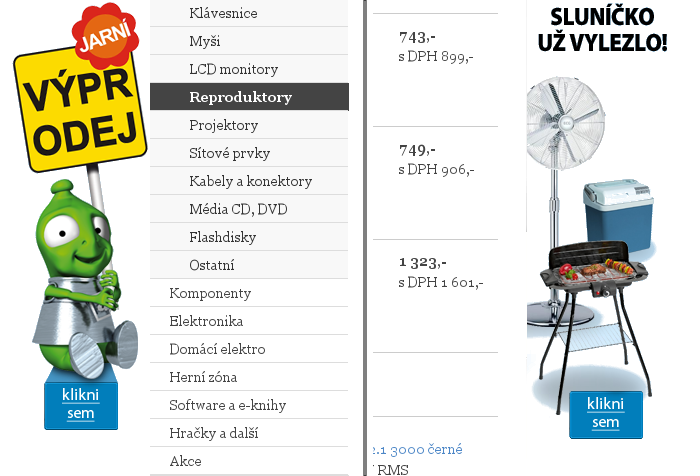
\includegraphics[scale=0.6]{images/image25.png}
	\end{center}
	\caption{Komponenta: Reklamní bannery fixně podél layoutu vlevo a~vpravo.}
	\label{imgBan2}
\end{figure}


\begin{figure}[h]
	\begin{center}
	
\includegraphics[scale=0.6]{images/image27.png}
	\end{center}
	\caption[Ukázka responzivní reklamy]{Komponenta: Horizontální obdoba bočních bannerů využívaná při responzivním designu.}
	\label{imgRes}
\end{figure}

%\chapter{Seznam použitých zkratek}
\nocite{*}
%\printglossaries
\printglossary[type=acronym,title=Seznam použitých zkratek]
%\begin{description}
%	\item[GUI] Graphical user interface
%	\item[XML] Extensible markup language
%\end{description}


% % % % % % % % % % % % % % % % % % % % % % % % % % % % 
% % Tuto kapitolu z~výsledné práce ODSTRAŇTE.
% % % % % % % % % % % % % % % % % % % % % % % % % % % % 
% 
% \chapter{Návod k~použití této šablony}
% 
% Tento dokument slouží jako základ pro napsání závěrečné práce na Fakultě informačních technologií ČVUT v~Praze.
% 
% \section{Výběr základu}
% 
% Vyberte si šablonu podle druhu práce (bakalářská, diplomová), jazyka (čeština, angličtina) a~kódování (ASCII, \mbox{UTF-8}, \mbox{ISO-8859-2} neboli latin2 a~nebo \mbox{Windows-1250}). 
% 
% V~české variantě naleznete šablony v~souborech pojmenovaných ve formátu práce\_kódování.tex. Typ může být:
% \begin{description}
% 	\item[BP] bakalářská práce,
% 	\item[DP] diplomová (magisterská) práce.
% \end{description}
% Kódování, ve kterém chcete psát, může být:
% \begin{description}
% 	\item[UTF-8] kódování Unicode,
% 	\item[ISO-8859-2] latin2,
% 	\item[Windows-1250] znaková sada 1250 Windows.
% \end{description}
% V~případě nejistoty ohledně kódování doporučujeme následující postup:
% \begin{enumerate}
% 	\item Otevřete šablony pro kódování UTF-8 v~editoru prostého textu, který chcete pro psaní práce použít -- pokud můžete texty s~diakritikou normálně přečíst, použijte tuto šablonu.
% 	\item V~opačném případě postupujte dále podle toho, jaký operační systém používáte:
% 	\begin{itemize}
% 		\item v~případě Windows použijte šablonu pro kódování \mbox{Windows-1250},
% 		\item jinak zkuste použít šablonu pro kódování \mbox{ISO-8859-2}.
% 	\end{itemize}
% \end{enumerate}
% 
% 
% V~anglické variantě jsou šablony pojmenované podle typu práce, možnosti jsou:
% \begin{description}
% 	\item[bachelors] bakalářská práce,
% 	\item[masters] diplomová (magisterská) práce.
% \end{description}
% 
% \section{Použití šablony}
% 
% Šablona je určena pro zpracování systémem \LaTeXe{}. Text je možné psát v~textovém editoru jako prostý text, lze však také využít specializovaný editor pro \LaTeX{}, např. Kile.
% 
% Pro získání tisknutelného výstupu z~takto vytvořeného souboru použijte příkaz \verb|pdflatex|, kterému předáte cestu k~souboru jako parametr. Vhodný editor pro \LaTeX{} toto udělá za Vás. \verb|pdfcslatex| ani \verb|cslatex| \emph{nebudou} s~těmito šablonami fungovat.
% 
% Více informací o~použití systému \LaTeX{} najdete např. v~\cite{wikilatex}.
% 
% \subsection{Typografie}
% 
% Při psaní dodržujte typografické konvence zvoleného jazyka. České \uv{uvozovky} zapisujte použitím příkazu \verb|\uv|, kterému v~parametru předáte text, jenž má být v~uvozovkách. Anglické otevírací uvozovky se v~\LaTeX{}u zadávají jako dva zpětné apostrofy, uzavírací uvozovky jako dva apostrofy. Často chybně uváděný symbol "{} (palce) nemá s~uvozovkami nic společného.
% 
% Dále je třeba zabránit zalomení řádky mezi některými slovy, v~češtině např. za jednopísmennými předložkami a~spojkami (vyjma \uv{a}). To docílíte vložením pružné nezalomitelné mezery -- znakem \texttt{\textasciitilde}. V~tomto případě to není třeba dělat ručně, lze použít program \verb|vlna|.
% 
% Více o~typografii viz \cite{kobltypo}.
% 
% \subsection{Obrázky}
% 
% Pro umožnění vkládání obrázků je vhodné použít balíček \verb|graphicx|, samotné vložení se provede příkazem \verb|\includegraphics|. Takto je možné vkládat obrázky ve formátu PDF, PNG a~JPEG jestliže používáte pdf\LaTeX{} nebo ve formátu EPS jestliže používáte \LaTeX{}. Doporučujeme preferovat vektorové obrázky před rastrovými (vyjma fotografií).
% 
% \subsubsection{Získání vhodného formátu}
% 
% Pro získání vektorových formátů PDF nebo EPS z~jiných lze použít některý z~vektorových grafických editorů. Pro převod rastrového obrázku na vektorový lze použít rasterizaci, kterou mnohé editory zvládají (např. Inkscape). Pro konverze lze použít též nástroje pro dávkové zpracování běžně dodávané s~\LaTeX{}em, např. \verb|epstopdf|.
% 
% \subsubsection{Plovoucí prostředí}
% 
% Příkazem \verb|\includegraphics| lze obrázky vkládat přímo, doporučujeme však použít plovoucí prostředí, konkrétně \verb|figure|. Například obrázek \ref{fig:float} byl vložen tímto způsobem. Vůbec přitom nevadí, když je obrázek umístěn jinde, než bylo původně zamýšleno -- je tomu tak hlavně kvůli dodržení typografických konvencí. Namísto vynucování konkrétní pozice obrázku doporučujeme používat odkazování z~textu (dvojice příkazů \verb|\label| a~\verb|\ref|).
% 
% \begin{figure}\centering
% 	
\includegraphics[width=0.5\textwidth, angle=30]{cvut-logo-bw}
% 	\caption[Příklad obrázku]{Ukázkový obrázek v~plovoucím prostředí}\label{fig:float}
% \end{figure}
% 
% \subsubsection{Verze obrázků}
% 
% % Gnuplot BW i~barevně
% Může se hodit mít více verzí stejného obrázku, např. pro barevný či černobílý tisk a~nebo pro prezentaci. S~pomocí některých nástrojů na generování grafiky je to snadné.
% 
% Máte-li například graf vytvořený v~programu Gnuplot, můžete jeho černobílou variantu (viz obr. \ref{fig:gnuplot-bw}) vytvořit parametrem \verb|monochrome dashed| příkazu \verb|set term|. Barevnou variantu (viz obr. \ref{fig:gnuplot-col}) vhodnou na prezentace lze vytvořit parametrem \verb|colour solid|.
% 
% \begin{figure}\centering
% 	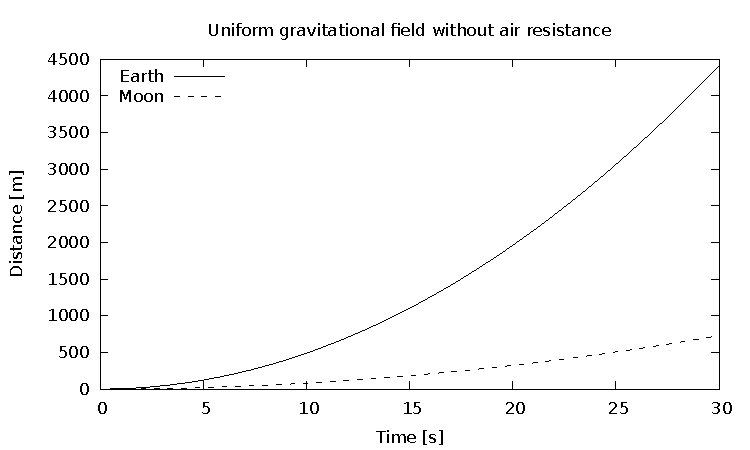
\includegraphics{gnuplot-bw}
% 	\caption{Černobílá varianta obrázku generovaného programem Gnuplot}\label{fig:gnuplot-bw}
% \end{figure}
% 
% \begin{figure}\centering
% 	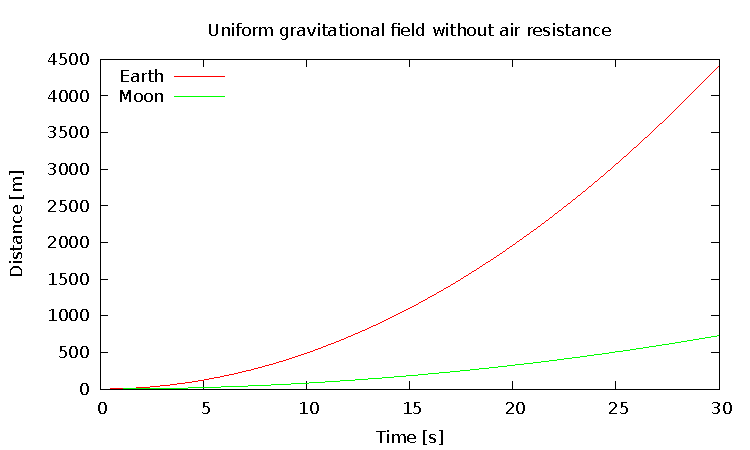
\includegraphics{gnuplot-col}
% 	\caption{Barevná varianta obrázku generovaného programem Gnuplot}\label{fig:gnuplot-col}
% \end{figure}
% 
% 
% \subsection{Tabulky}
% 
% Tabulky lze zadávat různě, např. v~prostředí \verb|tabular|, avšak pro jejich vkládání platí to samé, co pro obrázky -- použijte plovoucí prostředí, v~tomto případě \verb|table|. Například tabulka \ref{tab:matematika} byla vložena tímto způsobem.
% 
% \begin{table}\centering
% 	\caption[Příklad tabulky]{Zadávání matematiky}\label{tab:matematika}
% 	\begin{tabular}{|l|l|c|c|}\hline
% 		Typ		& Prostředí		& \LaTeX{}ovská zkratka	& \TeX{}ovská zkratka	\tabularnewline \hline \hline
% 		Text		& \verb|math|		& \verb|\(...\)|	& \verb|$...$|		\tabularnewline \hline
% 		Displayed	& \verb|displaymath|	& \verb|\[...\]|	& \verb|$$...$$|	\tabularnewline \hline
% 	\end{tabular}
% \end{table}
% 
% % % % % % % % % % % % % % % % % % % % % % % % % % % % 

\chapter{Obsah přiloženého CD}

%upravte podle skutecnosti

\begin{figure}
	\dirtree{%
		.1 readme.txt\DTcomment{stručný popis obsahu CD}.
		.1 src.
		.2 css-frameworky\DTcomment{zdrojové kódy testovaných CSS frameworků včetně komponenty}.
		.2 moduly-do-cms\DTcomment{zdrojové kódy modulů CSS preprocesorů do Venne:CMS}.		
		.2 thesis\DTcomment{zdrojová forma práce ve formátu \LaTeX{} včetně použitých obrázků}.
		.1 text\DTcomment{text práce}.
		.2 thesis.pdf\DTcomment{text práce ve formátu PDF}.
		.2 thesis.ps\DTcomment{text práce ve formátu PS}.
	}
\end{figure}

\end{document}
